%%%%%%%%%%%%%%%%%%%%%%%%%%%%%%%%%%%%%%%%%
% Thesis
% LaTeX Template
% Version 1.3 (21/12/12)
%
% This template has been downloaded from:
% http://www.latextemplates.com
%
% Original authors:
% Steven Gunn
% http://users.ecs.soton.ac.uk/srg/softwaretools/document/templates/
% and
% Sunil Patel
% http://www.sunilpatel.co.uk/thesis-template/
%
% License:
% CC BY-NC-SA 3.0 (http://creativecommons.org/licenses/by-nc-sa/3.0/)
%
% Note:
% Make sure to edit document variables in the Thesis.cls file
%
%%%%%%%%%%%%%%%%%%%%%%%%%%%%%%%%%%%%%%%%%

%----------------------------------------------------------------------------------------
%	PACKAGES AND OTHER DOCUMENT CONFIGURATIONS
%----------------------------------------------------------------------------------------

\documentclass[11pt, a4paper, oneside]{Thesis} % Paper size, default font size and one-sided paper

\graphicspath{{./Pictures/}} % Specifies the directory where pictures are stored

\usepackage[square, numbers, comma, sort&compress]{natbib} % Use the natbib
%reference package - read up on this to edit the reference style; if you want
%text (e.g. Smith et al., 2012) for the in-text references (instead of
%numbers), remove 'numbers'
\usepackage{isomath}
\usepackage{paralist}
\usepackage{tabulary}
\hypersetup{urlcolor=blue, colorlinks=true} % Colors hyperlinks in blue -
%change to black if annoying
\title{\ttitle} % Defines the thesis title - don't touch this


% Use double bar notations: http://tex.stackexchange.com/questions/43008/absolute-value-symbols/43009#43009
\usepackage{mathtools}
\DeclarePairedDelimiter\abs{\lvert}{\rvert}%
\DeclarePairedDelimiter\norm{\lVert}{\rVert}%

% Swap the definition of \abs* and \norm*, so that \abs
% and \norm resizes the size of the brackets, and the
% starred version does not.
\makeatletter
\let\oldabs\abs
\def\abs{\@ifstar{\oldabs}{\oldabs*}}
%
\let\oldnorm\norm
\def\norm{\@ifstar{\oldnorm}{\oldnorm*}}
\makeatother
% End of double bar notations

\DeclareMathOperator*{\argminold}{\arg\!\min}
\DeclareMathOperator*{\argmaxold}{\arg\!\max}

% \usepackage{hyperref}
\usepackage[nomain,acronym,xindy,toc]{glossaries}
\renewcommand*{\glstextformat}[1]{\textcolor{black}{#1}}
\makeglossaries
\usepackage[xindy]{imakeidx}
\makeindex

\usepackage{templates/math_shorthands}

\begin{document}
% !TEX root = main.tex

% A C R O N Y M S

\newacronym{ar}{AR}{Autoregressive}

\newacronym{aic}{AIC}{Akaike Information Criterion}

\newacronym{bic}{BIC}{Bayesian Information Criterion}

\newacronym{cusum}{CUSUM}{Cumulative Sum}

\newacronym{dr}{DR}{Dimensionality Reduction}

\newacronym{har}{HAR}{Human Activity Recognition}

\newacronym{gmm}{GMM}{Gaussian Mixture Model}

\newacronym{hmm}{HMM}{Hidden Markov Model}

\newacronym{icss}{ICSS}{Iterated Cumulative Sums of Squares}

\newacronym{iid}{i.i.d.}{independently and identically distributed}

\newacronym{isvdd}{I-SVDD}{Incremental Support Vector Data Description}

\newacronym{kl}{KL}{Kullback-Leibler}

\newacronym{kliep}{KLIEP}{Kullback-Leibler Importance Estimation Procedure}

\newacronym{kkt}{KKT}{Karush–-Kuhn–-Tucker}

\newacronym{mle}{MLE}{Maximum Likelihood Estimates}

\newacronym{mosum}{MOSUM}{Moving Sum}

\newacronym{nu-svm}{$\nu$-SVM}{$\nu$-Support Vector Machine}

\newacronym{occ}{OCC}{One-Class Classification}

\newacronym{oc-svm}{OC-SVM}{One-Class Support Vector Machine}

\newacronym{pca}{PCA}{Principal Component Analysis}

\newacronym{pdf}{PDF}{Probability Density Function}

\newacronym{qp}{QP}{Quadratic Programming}

\newacronym{rbf}{RBF}{Radial Base Function}

\newacronym{roc}{ROC}{Receiver-Operating Characteristic}

\newacronym{rt}{RT}{Ratio-Thresholding}

\newacronym{sv}{SV}{Support Vector}

\newacronym{svc}{SVC}{Support Vector Classifier}

\newacronym{svcpd}{SVCPD}{Support Vector based Change Point Detection}

\newacronym{svdd}{SVDD}{Support Vector Data Description}

\newacronym{svm}{SVM}{Support Vector Machine}

\newacronym{swab}{SWAB}{Sliding Window And Bottom-up}

\newglossaryentry{changeFinder}
{
  name=changeFinder,
  description={is a unifying framework proposed by Tackeuchi and Yamanishi \cite{takeuchi2006unifying} which combines outlier detection and change detection.}
}

\frontmatter % Use roman page numbering style (i, ii, iii, iv...) for the pre-content pages

\setstretch{1.3} % Line spacing of 1.3

% Define the page headers using the FancyHdr package and set up for one-sided printing
\fancyhead{} % Clears all page headers and footers
\rhead{\thepage} % Sets the right side header to show the page number
\lhead{} % Clears the left side page header

\pagestyle{fancy} % Finally, use the "fancy" page style to implement the FancyHdr headers

\newcommand{\HRule}{\rule{\linewidth}{0.5mm}} % New command to make the lines in the title page

\newcommand{\TODO}[1]{\emph{\textbf{*** TODO: {#1} ***}}}

\ExplSyntaxOn
\newcommand\latinabbrev[1]{
  \peek_meaning:NTF . {% Same as \@ifnextchar
    #1\@}%
  { \peek_catcode:NTF a {% Check whether next char has same catcode as \'a, i.e., is a letter
      #1.\@\ }%
    {#1.\@\ }}}
\ExplSyntaxOff

%Omit final dot from each def.
\def\eg{\latinabbrev{e.g}}
\def\etal{\latinabbrev{\textit{et al}}}
\def\etc{\latinabbrev{etc}}
\def\ie{\latinabbrev{i.e}}

% PDF meta-data
\hypersetup{pdftitle={\ttitle}}
\hypersetup{pdfsubject=\subjectname}
\hypersetup{pdfauthor=\authornames}
\hypersetup{pdfkeywords=\keywordnames}

%----------------------------------------------------------------------------------------
%	TITLE PAGE
%----------------------------------------------------------------------------------------

\begin{titlepage}
\begin{center}

\textsc{\LARGE \univname}\\[1.5cm] % University name
\textsc{\Large Doctoral Thesis}\\[0.5cm] % Thesis type

\HRule \\[0.4cm] % Horizontal line
{\huge \bfseries \ttitle}\\[0.4cm] % Thesis title
\HRule \\[1.5cm] % Horizontal line

\begin{minipage}{0.4\textwidth}
\begin{flushleft} \large
\emph{Author:}\\
\href{http://www.johnsmith.com}{\authornames} % Author name - remove the \href bracket to remove the link
\end{flushleft}
\end{minipage}
\begin{minipage}{0.4\textwidth}
\begin{flushright} \large
\emph{Supervisor:} \\
\href{http://www.jamessmith.com}{\supname} % Supervisor name - remove the \href bracket to remove the link
\end{flushright}
\end{minipage}\\[3cm]

\large \textit{A thesis submitted in fulfilment of the requirements\\ for the degree of \degreename}\\[0.3cm] % University requirement text
\textit{in the}\\[0.4cm]
\groupname\\\deptname\\[2cm] % Research group name and department name

{\large \today}\\[4cm] % Date
%\includegraphics{Logo} % University/department logo - uncomment to place it

\vfill
\end{center}

\end{titlepage}

%----------------------------------------------------------------------------------------
%	DECLARATION PAGE
%	Your institution may give you a different text to place here
%----------------------------------------------------------------------------------------

\Declaration{

\addtocontents{toc}{\vspace{1em}} % Add a gap in the Contents, for aesthetics

I, \authornames, declare that this thesis titled, '\ttitle' and the work presented in it are my own. I confirm that:

\begin{itemize}
\item[\tiny{$\blacksquare$}] This work was done wholly or mainly while in candidature for a research degree at this University.
\item[\tiny{$\blacksquare$}] Where any part of this thesis has previously been submitted for a degree or any other qualification at this University or any other institution, this has been clearly stated.
\item[\tiny{$\blacksquare$}] Where I have consulted the published work of others, this is always clearly attributed.
\item[\tiny{$\blacksquare$}] Where I have quoted from the work of others, the source is always given. With the exception of such quotations, this thesis is entirely my own work.
\item[\tiny{$\blacksquare$}] I have acknowledged all main sources of help.
\item[\tiny{$\blacksquare$}] Where the thesis is based on work done by myself jointly with others, I have made clear exactly what was done by others and what I have contributed myself.\\
\end{itemize}

Signed:\\
\rule[1em]{25em}{0.5pt} % This prints a line for the signature

Date:\\
\rule[1em]{25em}{0.5pt} % This prints a line to write the date
}

\clearpage % Start a new page

%----------------------------------------------------------------------------------------
%	QUOTATION PAGE
%----------------------------------------------------------------------------------------

\pagestyle{empty} % No headers or footers for the following pages

\null\vfill % Add some space to move the quote down the page a bit

\textit{``Thanks to my solid academic training, today I can write hundreds of words on virtually any topic without possessing a shred of information, which is how I got a good job in journalism."}

\begin{flushright}
Dave Barry
\end{flushright}

\TODO{Find nice quote}

\vfill\vfill\vfill\vfill\vfill\vfill\null % Add some space at the bottom to position the quote just right

\clearpage % Start a new page

%----------------------------------------------------------------------------------------
%	ABSTRACT PAGE
%----------------------------------------------------------------------------------------

\addtotoc{Abstract} % Add the "Abstract" page entry to the Contents

\abstract{\addtocontents{toc}{\vspace{1em}} % Add a gap in the Contents, for aesthetics

The Thesis Abstract is written here (and usually kept to just this page). The page is kept centered vertically so can expand into the blank space above the title too\ldots
}

\clearpage % Start a new page

%----------------------------------------------------------------------------------------
%	ACKNOWLEDGEMENTS
%----------------------------------------------------------------------------------------

\setstretch{1.3} % Reset the line-spacing to 1.3 for body text (if it has changed)

\acknowledgements{\addtocontents{toc}{\vspace{1em}} % Add a gap in the Contents, for aesthetics

The acknowledgements and the people to thank go here, don't forget to include your project advisor\ldots
}
\clearpage % Start a new page

%----------------------------------------------------------------------------------------
%	LIST OF CONTENTS/FIGURES/TABLES PAGES
%----------------------------------------------------------------------------------------

\pagestyle{fancy} % The page style headers have been "empty" all this time, now use the "fancy" headers as defined before to bring them back

\lhead{\emph{Contents}} % Set the left side page header to "Contents"
\tableofcontents % Write out the Table of Contents

\lhead{\emph{List of Figures}} % Set the left side page header to "List of Figures"
\listoffigures % Write out the List of Figures

\lhead{\emph{List of Tables}} % Set the left side page header to "List of Tables"
\listoftables % Write out the List of Tables

% %----------------------------------------------------------------------------------------
% %	ABBREVIATIONS
% %----------------------------------------------------------------------------------------

% \clearpage % Start a new page

% \setstretch{1.5} % Set the line spacing to 1.5, this makes the following tables easier to read

% \lhead{\emph{Abbreviations}} % Set the left side page header to "Abbreviations"
% \listofsymbols{ll} % Include a list of Abbreviations (a table of two columns)
% {
% \textbf{LAH} & \textbf{L}ist \textbf{A}bbreviations \textbf{H}ere \\
% %\textbf{Acronym} & \textbf{W}hat (it) \textbf{S}tands \textbf{F}or \\
% \textbf{PCA} & \textbf{P}rinciple \textbf{C}omponent \textbf{A}nalysis
% }

%----------------------------------------------------------------------------------------
% GLOSSARIES
%----------------------------------------------------------------------------------------

\clearpage

\lhead{\emph{Acronyms}}

\printglossaries


% %----------------------------------------------------------------------------------------
% %	PHYSICAL CONSTANTS/OTHER DEFINITIONS
% %----------------------------------------------------------------------------------------

% \clearpage % Start a new page

% \lhead{\emph{Physical Constants}} % Set the left side page header to "Physical Constants"

% \listofconstants{lrcl} % Include a list of Physical Constants (a four column table)
% {
% Speed of Light & $c$ & $=$ & $2.997\ 924\ 58\times10^{8}\ \mbox{ms}^{-\mbox{s}}$ (exact)\\
% % Constant Name & Symbol & = & Constant Value (with units) \\
% }

%----------------------------------------------------------------------------------------
%	SYMBOLS
%----------------------------------------------------------------------------------------

\clearpage % Start a new page

\lhead{\emph{Symbols}} % Set the left side page header to "Symbols"

\listofnomenclature{lll} % Include a list of Symbols (a three column table)
{
$a$ & distance & m \\
$P$ & power & W (Js$^{-1}$) \\
% Symbol & Name & Unit \\

& & \\ % Gap to separate the Roman symbols from the Greek

$\omega$ & angular frequency & rads$^{-1}$ \\
% Symbol & Name & Unit \\
}

%----------------------------------------------------------------------------------------
%	DEDICATION
%----------------------------------------------------------------------------------------

\clearpage
\setstretch{1.3} % Return the line spacing back to 1.3

\pagestyle{empty} % Page style needs to be empty for this page

\dedicatory{For/Dedicated to/To my\ldots} % Dedication text

\addtocontents{toc}{\vspace{2em}} % Add a gap in the Contents, for aesthetics

%----------------------------------------------------------------------------------------
%	THESIS CONTENT - CHAPTERS
%----------------------------------------------------------------------------------------

\mainmatter % Begin numeric (1,2,3...) page numbering

\pagestyle{fancy} % Return the page headers back to the "fancy" style

% Include the chapters of the thesis as separate files from the Chapters folder
% Uncomment the lines as you write the chapters

% !TEX root = ../main.tex
% Chapter 1

\chapter{Introduction}

\label{Chapter1} % For referencing the chapter elsewhere, use~\ref{Chapter1}

\lhead{Chapter 1. \emph{Introduction}} % This is for the header on each page - perhaps a shortened title

%----------------------------------------------------------------------------------------

\section{Outline}
\emph{Not intented for the reader.}
\begin{itemize}
  \item Context of research (\gls{har}), real-world applications
  \item Current methods, wrapper vs. filter methods
  \item Problem statement with current filter methods (which follows from \Cref{Chapter3} which goes in-depth with methods).
  \item Purpose of this research. E.g. "Find a better algorithm for short-activity segmentation"
  \item Provide the \emph{motivation} for this approach
  \item Relate to real-world applications
  \item Outline for rest of the thesis
\end{itemize}

-- Overall todo's --
\begin{itemize}
  \item \TODO{The term \emph{emperical data/distruction} is nowhere used in the thesis. or: Emperical cumulative distribution. Especially Chapter 2.}
  \item \TODO{Check for ``tang-constructions'': saying to much in a single sentence.}
  \item \TODO{Overall: meer focus op de \emph{waarom} vraag/antwoord bij keuzes. Bouwt aan motivatie en context van het geheel.}
  \item \TODO{Nu staat nog veel (met name Chapter 2) in ``aantekening'' style; ombouwen naar uitleggen, lezer begeleiden, duiden, verlaren etc.}
  \item \TODO{Test moet condenser: bepalen wat er uit gelaten mag worden.}
\end{itemize}

\begin{figure}
  \centering
    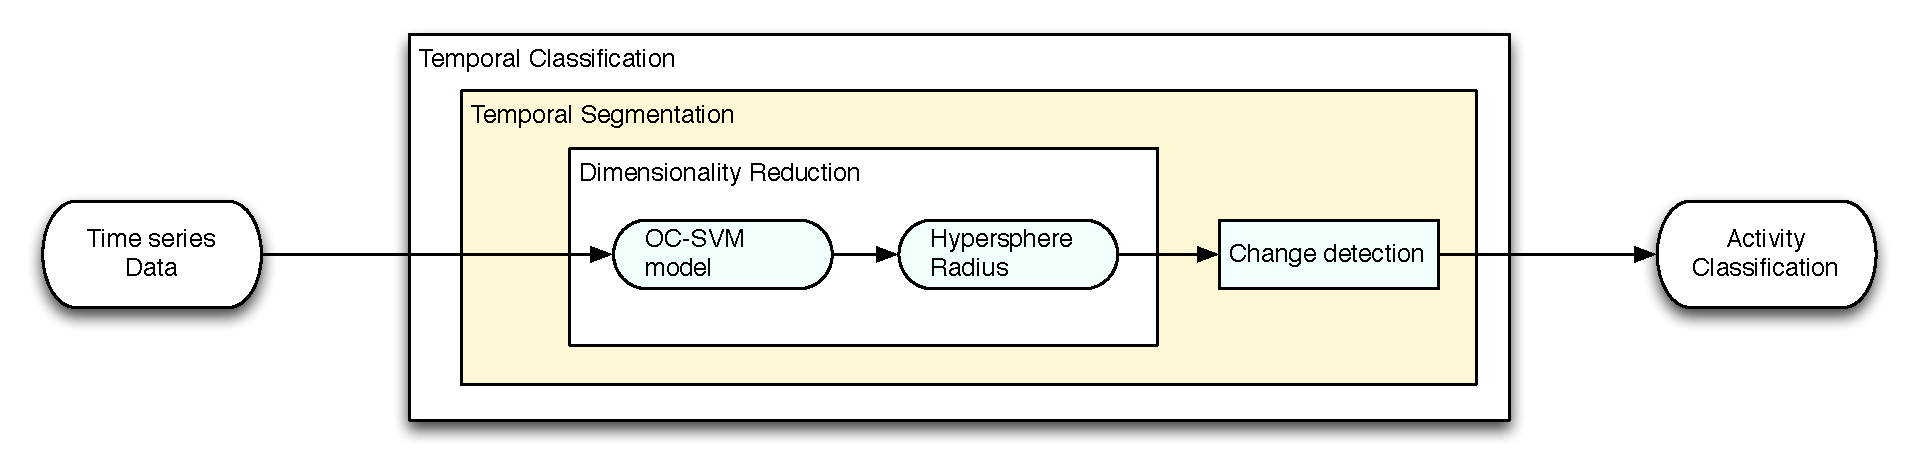
\includegraphics[width=\textwidth,height=\textheight,keepaspectratio]{./Figures/chapter1/thesis_goal.pdf}
  \caption[Thesis goal]{The goal of this thesis. The scope of this thesis is Temporal Segmentation, which can be useful in the context of Temporal Classification. Given a data set, we apply the construction of \gls{oc-svm} models as a form of dimensionality reduction. Using the reduced representation, being the radius $R$ of the constructed hypersphere, we apply direct change detection methods. The detected change points can support the classification of homogeneous segments of data.}
  \label{fig:thesis_goal}
\end{figure}


\begin{itemize}
  \item Begin with hook, statement, to draw attention
  \item Cite previous work and explain why new research was necessary.
  \item Statement of the goal of the thesis: why?
  \item Context to understand background of goal and the significance
  \item Acknowledgement of previous research and context
  \item Explain scope: what will be, and wont be discussed
  \item Verbal table of contents
  \item
\end{itemize}

Introduction to the introduction \\
Context \\
Restatement of problem and significance (echo of opening, but now with the context) \\
Restatement of the response \\
Roadmap \\

\section{Intro to intro}
With the wide availability of smartphones and built-in inertial sensors, more and more applications of \gls{har} are introduced.
Many approaches to recognizing the performed activity rely on classification of recorded data, which can be done online or in batches after the performance.
Often an time-windowed based approach is used, which feeds short consecutive segments of data through a model construction phase.
The constructed model is used to determine what (earlier learned) activity is performed.
Besides the explicit classification of the data, an implicit result is a segmentation of performed activities over time.

In this thesis the goal is to find the temporal segmentation of time series data explicitly, prior to the classification of the activities.
This is done under the assumption that it could be beneficial for classification methods to possess this explicit segmentation, since the model construction phase can use more data than the time-windowed approach would allow.
To find the temporal segmentation, we rely on change detection in time series data.
In the context of this research, this time series data consist of recordings from inertial sensors found in smartphones, during the performance of human activities.
We have recorded both in- and outdoor activities in an uncontrolled environment and in a continuous manner.

For the change detection algorithm we have used a special form of \gls{svm}, the \gls{oc-svm} based \gls{svdd} as introduced by Tax~\cite{tax2001one}.
This method models the data under consideration in the shape of a high-dimensional hypersphere.
From this hypersphere the radius is extracted, since a change in data characteristics (resulting from a change in performed activity) should result in a change of radius.





\section{Thesis structure}
The structure of this thesis is as follows.
In \Cref{Chapter2} a literature review is provided.
We will look at the different interpretations and implementations for change, novelty, and outlier detection.
Previous work in the field of \gls{har} is discussed and we end with existing applications of \glspl{svm} to change detection.
The next chapter further analyses \glspl{svm} and two implementations of \glspl{oc-svm}.
It relates the properties of the constructed \gls{oc-svm} models to change detection in time series data.
That relation is applied to our problem formulation in \Cref{Chapter4}, where we construct our change detection method, based on the work of Camci~\cite{camci2010change}.
The two following chapters apply the method to both artificial and real-world data.
\Cref{Chapter5} show the objective performance of the method to artificial constructed data.
In \Cref{Chapter6} we apply the method to our self-recorded real-world data.
We show the ability of detecting change in \gls{har} data, recorded by inertial sensors.
This thesis is conclused in \Cref{Chapter7}, in which we reflect on the performed research and state possibilities for feature research.
% !TEX root = ../main.tex
% Chapter 2

\chapter{Literature review}

\label{Chapter2} % For referencing the chapter elsewhere, use \ref{Chapter2}

\lhead{Chapter 2. \emph{Literature review}} % This is for the header on each page - perhaps a shortened title

%----------------------------------------------------------------------------------------
\section{Outline}
\begin{itemize}
  \item Literature review about Temporal Segmentation (previous draft was more about classification)
  \item Consider methods for the context of filter-methods for classification
  \item Take a loot at 3-4 different kind of methods for change detection:
    \begin{itemize}
      \item Introduction with a lot of techniques
      \item Explain why look at a few
      \item CUSUM - or other more traditional methods
      \item Density-ratio estimation
      \item Support Vector Machines (?) - if there are more sources about this
      \item (Dimensionality reduction)
    \end{itemize}
  \item With each method, shortly look at characteristics, strengths and weaknesses and consider applicability to accelerometer sensor data
\end{itemize}


% \section{Statistical framework}\label{statistical-framework}
% Many applications require the detection of time points at which the underlying properties of a system change.
% This problem thus has received a lot of attention in the fields of data mining, etc... *** list and refs ***.
% Often this problem is formulated in a statistical framework, by inspecting the data generating PDF (Probability Density Function) of the time series data.
% A change point is then defined as a significant change in the properties of the PDF, such as the mean and variance.

% The widely used CUSUM (cumulative sum) method by Basseville \etal \cite{basseville1993detection}, and the GLR (Generalized Likelihood Ratio) by Gustafsson \cite{gustafsson1996marginalized,gustafsson2000adaptive} take this approach.
% The former originates from control methods for detection from bench marks.
% The latter compares the logarithm of the likelihood ratio over two consecutive intervals.
% These two methods is discussed and analyzed in section \ref{cusum-glr}.

% The GLR method, as with others, relies on pre-specified parametric model assumptions and considers the data be independent over time, which makes it less flexible to real-world applications.
% The proposed methods by Kawahara \etal \cite{kawahara2009change} and Lui \etal \cite{liu2013change} try to overcome these problems by estimating the \emph{ratio} between the PDF, instead of estimating each PDF.
% This approach is discussed and analyzed in section \ref{density-ratio}.

% The density-estimation methods, as with the GLR, rely on the log-likelihood ratio between PDFs.
% The method of Camci \cite{camci2010change} takes an other approach within the statistical framework, by using a SVM (Support Vector Machine).
% One problem it tries to overcome is the (claimed) weakness of many methods to detect a decrease in variance.
% The method represents the distribution over the data points as a hyper-sphere in a higher dimension using kernel trick.
% A change in the PDF is represented by a change in the radius of this sphere.
% Section \ref{svm} discusses the SVM-method.

% The final method under consideration, change detection via (intrinsic) dimensionality reduction, takes a different point of view.
% Opposed to the other discussed methods, dimensionality reduction is framed in the MDL (Minimum Description Length) framework.
% It uses the estimated underlying number of parameters of the time series as a model for change detection.
% Section \ref{dim-reduction} discuses this method.



%----------------------------------------------------------------------------------------
% CUSUM and GLR
% !TEX root = ../../main.tex
\section{CUSUM and GLR}\label{cusum-glr}

*** read book Basseville \cite{basseville1993detection} ***


\subsection{CUSUM}
Non-Bayesian change detection algorithm (thus: no prior distribution believe available for the change time).

The CUSUM (cumulative sum) method is developed by Page \cite{page1954continuous} for the application of statistical quality control (it is also known as a control chart).

Primary for detection of mean shift.

The MOSUM of squares test for monitoring variance changes \cite{hsu2007mosum}.

Use of Cumulative Sums of Squares for Retrospective Detection of Changes of Variance \cite{inclan1994use}


\subsection{GLR}
Also: maximum-likelihood estimation. ``When applied to a dataset and a given statistical model, it provides estimates for the model's parameters.''

%----------------------------------------------------------------------------------------
% Density Ratio Estimation
% !TEX root = ../../main.tex
\section{Change-detection by Density-Ratio Estimation}\label{sec:density-ratio}

% Papers:
% \begin{itemize}
%   \item Change-Point Detection in Time-Series Data by Direct Density-Ratio Estimation, 2009, 45 refs \cite{kawahara2009change}
%   \item Change-Point Detection in Time-Series Data by Relative Density-Ratio Estimation, 2013, 3 refs \cite{liu2013change}
%   \item Density ratio estimation in machine learning (Book), 2009, 24 refs \cite{sugiyama2012density}
%   \item Direct importance estimation for covariate shift adaptation, 2008, 84 refs \cite{sugiyama2008direct}
% \end{itemize}

% Formulate the problem of detecting change in the statistical framework.
% Consider the probability distributions from which two consecutive segments of time series around a target time point are generated.
% When the disitrubtions differ significantly the target time point is regarded as a change point.




% CUSUM (cumulative sum) \cite{basseville1993detection} and GLR (generalized likelihood ratio)


% The distribution over the values of time series data can be represented with a probability density function (pdf).
% Two sections of a time series data can be generated with the same underlying pdf or each with a different.

Many approaches to detect change points monitor the logarithm of the likelihood ratio between two consecutive intervals.
A change point is regarded to be the moment in time when the underlying probabilistic generation function changes.
Some methods which rely on this are novelty detection, maximum-likelihood estimation and online learning of autoregressive models \cite{kawahara2009change}.
A limitation of these methods is that they rely on pre-specified parametric models.
Nonparametric models, for which the number and nature of the parameters are undetermined, for density estimation have been proposed, but it is said to be a hard problem \cite{hardle2004nonparametric, sugiyama2012density}.
A solution to this is to estimate the \emph{ratio} of probabilities instead of the probabilities themselves.
One of the recent methods to achieve this is the \gls{kliep} by Sugiyama \etal \cite{sugiyama2008direct}.

The proposed method by Kawahara and Sugiyama~\cite{kawahara2009change} uses an online version of the \gls{kliep} algorithm.
It considers \emph{sequences} of samples (rather than samples directly) because the time series samples are generally not independent over time.
The method detects change by monitoring the logarithm of the likelihood ratio between densities of reference (past) and test (current) time intervals.
If it exceeds a predetermined threshold value, the beginning of the test interval is marked as a change point.

Since the density ratio is unknown, it needs to be estimated.
The naive approach is to estimate it using estimated densities of the two intervals.
Since this is known to be a hard problem and sensitive for errors, the solution would be to estimate the ratio directly.

The method by Liu \etal \cite{liu2013change} estimates the ratio of probabilities directly, instead of estimating the densities explicitly.
Other methods using ratio-estimation are the Unconstrained Least-Squares Importance Fitting (uLSIF) method \cite{kanamori2009least}, and an extension which possesses a superior nonparametric convergence property: Relative uLSIF (RuLSIF) \cite{yamada2013relative}.

%----------------------------------------------------------------------------------------
% Support Vector Machines
% !TEX root = ../../main.tex
\section{Change-detection by Support Vector Machines}\label{svm}

Introduced by Vapnik \cite{vapnik1998statistical, vapnik1999nature}, Support Vector Machines offer a way to segment, and classify, linear separable data.
This technique can also be applied to estimate density functions of given time series \cite{weston1999support}.
When combined with a mapping function, which maps the data from the input space $I$ to a higher dimension feature space $F$, the input data can be non-linear separable.
The linear hyperplane, which segments the data in the feature space $F$, yields to a non-linear segmentation in the lower-dimensional input space $I$.
Instead of explicitly mapping the input data to the higher dimensional space, a kernel function can be used.
This kernel function can calculate values of the feature space directly, without the need to first map the input values to this space.
This process is referred to as the kernel trick.

The method of Camci \cite{camci2010change} uses one-class support vector machines to segment time series data.
For the current interval a hyper-sphere is constructed, using the kernel trick, which circumscribes all the data.
To cope with possible errors or outliers a soft-margin is applied.
The data can thus be represented using a center $c_1$ and radius $r_1$ of the hyper-sphere.
New data points are consecutively mapped from the input space to the feature space.
The retrieved (high dimension) data point can be in- or outside the earlier constructed hyper-sphere, thereby giving information about a possible change point.



\subsection{One-class Support Vector Machine}
*** This section is too detailed for the Literature Review, but keep it for now ***


*** Replace with / add information from summary in \ref{svm-explained}. ***

The proposed method of Camci \cite{camci2010change} uses a one-class support vector machine to segment time series data.
One-class SVMs are used to describe the current data under consideration, by assuming all data points are from the same class \cite{tax2001one}.
The class is described by a spherical boundary around the data with center $c$ and radius $r$, such that the volume is minimized.
Following the definition of Camci \cite{camci2010change}, the class description is obtained by minimizing $r^2$:
\begin{equation}
  \mathrm{Min}\ r^2
\end{equation}
\begin{equation}
  \mathrm{Subject\ to} : \|\mathbf{x}_i - \mathbf{c}\|^2 \le r^2\ \forall i,\ \mathbf{x}_i : i \mathrm{th\ data\ point}
\end{equation}

To be able to handle outliers in the input data, a penalty cost function $\varepsilon_i$ for each outlier can be added.

*** Add new function and constraints? ***

Using this one-class SVM formulation, differences between two (consecutive) windows of data points with size $w$ can be obtained.
The first window is used as the input set, $h_1$ and the second as the test set $h_t$.
For the first window a one-class SVM is constructed, yielding in a representation by $c_1$ and $r_1$.
When the data points of the second window belong to the same class, the representation of that one-class SVM would equal the first:
\begin{equation}
\begin{aligned}
  c_1 = c_2, & &  r_1 = r_2
\end{aligned}
\end{equation}

*** First tell more about (underlying) probability density functions, to relate to other methods ***

In case the second window of data points does not belong to the same class, i.e. the probability density function that describes the data differs from the first, the describing values of the second window will differ from the first.
The amount of difference can be expressed by a dissimilarity measure over the representations.
When the dissimilarity between the two windows exceeds some predefined threshold $th$, there exists a change point between the windows.

This process can be visualized as done in *** insert figure of four circles ***. The second window, $h_2$ can be constructed from the first by e.g. a shift of one data point. *** explain data point positions by circle ***.

Note that a difference in the SVM center $c$ or radius $r$ represent a change in the mean and variance, respectively.



%----------------------------------------------------------------------------------------
% Dimensionality reduciton
% !TEX root = ../../main.tex
\section{Change-detection by Dimensionality Reduction / Covariance structure}\label{dim-reduction}



% !TEX root = ../main.tex
% Chapter 3

\chapter{Change detection by Support Vector Machines}

\label{Chapter3} % For referencing the chapter elsewhere, use~\ref{Chapter3}

\lhead{Chapter 3. \emph{Change detection by Support Vector Machines}} % This is for the header on each page - perhaps a shortened title

This chapter discusses the concepts and algorithms that will be used as a basis for the proposed method, as introduced in \Cref{Chapter4}.
The first section formulates the problem of change detection and relates it to outlier and novelty detection.
It transforms the traditional problem of outlier detection into change detection for times series data.
In \Cref{sec:one_class_classification} the problem of \acrlong{occ} is explained and discusses a number of implementations.
In the final sections of this chapter, \Cref{sec:one_class_svm}, two \gls{svm}-based \gls{occ} methods, \gls{nu-svm} and \gls{svdd}, and the influence of model parameters are further discussed in detail.

% !TEX root = ../../main.tex
\section{Change Detection in Time Series}\label{sec:change_detection_time_series}
\TODO{Write section introduction} \\
\emph{The section should relate the problem of outlier detection to change detection.
It should transform the traditional problem formulation to that of time series data.
Build to one-class classification, which can be used for outlier detection}

\subsection{Relation to outlier detection}
The problems of outlier and novelty detection, segmentation, and change detection are closely related.
The terminology depends on the field of application, but there are subtle differences.
The problem of outlier detection is concerned with finding data objects in a data set which have small resemblance with the majority of the data objects.
These objects can be regarded as erroneous measurements.
In the case of novelty detection these objects are considered to be member of a new class of objects.
The unifying framework of Takeuchi and Yamanishi \cite{takeuchi2006unifying}, \gls{changeFinder}, creates a two stage process expressing change detection in terms of outlier detection.
The first stage determines the outliers in a time series by giving a score based on the deviation from a learned model, and thereby creates a new time series.
The second stage runs on that new created time series and calculates a average over a window of the outlier scores.
The problem of change detection is then reduced to outlier detection over that average-scored time series.
The implementation by Camci \cite{camci2010change}, \gls{svcpd}, implements outlier detection with the \gls{svdd} algorithm to detect changes in mean and variance.

\subsection{Problem formulation}\label{subsec:change_detection_problem_formulation}
\TODO{Note: the following block is copied from~\ref{sec:method_change_indication}} \\
The problem of change point detection can be formulated using different type of models, as discussed in~\ref{subsec:segmentation}.
The methods by Takeuchi and Yamanishi \cite{takeuchi2006unifying} and Camci \cite{camci2010change} use the following formulation for change detection, which we will also use for our problem formulation.
The algorithm searches for sudden changes in the time series data.
In other words, slowly changing properties in the data are not considered to be changes.
Considered a time series $x_1 x_1 \dots$, which is drawn from a stochastic process $p$.
Each $x_t$ (t = 1, 2, \dots) is a $d$-dimensional real valued vector and $p$ a probability density function of the sequence $x_1 x_2 \dots$.
Assume $p$ can be decomposed in two different \gls{iid} stationary stochastic processes $p^1$ and $p^2$ and are one-dimensional Gaussian density functions.
For a time point $a$ data points for which $t < a$ are drawn from $p^1 = N(\mu_1, \sigma_1^2)$ and for $t \geq a$ from $p^2 = N(\mu_2, \sigma_a^2)$.
If $p^1$ and $p^2$ are different, then the time point $t = a$ is a \emph{change point}.
In \cite{takeuchi2006unifying} the similarity between the stochastic processes are expressed by the \gls{kl} divergence $D(p^2||p^1)$.
It is observed that this measure is not able to detect a change by decrease in variance \cite{takeuchi2006unifying,camci2010change}.
This problem is the motivation for Camci \cite{camci2010change} to create the \gls{svcpd} algorithm.

The definition of change point being sudden changes in the time series data is in line with the search of changes in activities.
Since we are only interested in different activities (which are represented by sudden changes), slight changes within an activity are not of interest.
\Cref{sec:sensor_data_characteristics} discusses the representation of activities and changes between them in the data in more detail.

\TODO{add more formal definition or analysis of change detection}

-- Literature --

``Online segmentation of time series based on polynomial least-squares approximations'', \cite{fuchs2010online}. 25, 2010 \\

% \subsection{General framework for outlier detection}
% In \cite{schubert2012local} a general framework for outlier detection is proposed.
% The authors compare existing methods and identified the common building block of the algorithms.
% The focus is on unsupervised methods, using information from a local selection of data objects for the detection of outliers.
% The following common algorithmic building blocks are identified:

% \begin{enumerate}
%   \item Context: a ``local'' context of an object $o$ for model building
%   \item Model: the method used for building the model
%   \item Reference: a ``reference'' context of object $o$ for model comparison
%   \item Comparison: the method used for model comparison
%   \item Normalization: a (global) normalization procedure
% \end{enumerate}

% Here the \emph{context} and \emph{reference} are sets of objects used for model building and model comparison, respectively.


% \subsection{Regression, Classification, etc}

% General framework of outlier detection, change detection in context of (simple?) regression, classification.

% \subsection{M-estimators}
% \TODO{Move this section to somewhere in the end; is specification/extension, not base material}
% To make a method less sensitive to outliers (in the training data) techniques from robust statistics are applied.
% The term \emph{robustness} has many interpretations, one of them that it ``signifies insensi­tivity to small deviations from the [prior] assumptions [about the underlying situation]'', according to Huber \cite{huber2009robust}.
% Methods have been proposed to apply robust statistics in the form of M-estimators to \glspl{svm}, such as \cite{choi2009least,chen2004m,suykens1999least}.

% \TODO{Question: do slack-variables (allowance of outliers) make SVM robust?}
% !TEX root = ../../main.tex
\section{One-Class Classification}\label{sec:one_class_classification}
As discussed in the previous section, change detection in time series can be implemented using outlier, or novelty, detection.
To regard a data point as an outlier, there must be a model of the normal time series data and a (dis)similiarity measure defined over the model and data objects.
When a data point differs enough from the created model, it can be labeled as an outlier.
The class of \gls{occ} algorithms is especially designed for that purpose.
The algorithms build up a model of the data, assuming only normal data objects are available (or a very limited amount of example outlier data objects).
This is also known as novelty detection or semi-supervised detection and is of Type 3 in the system by Hodge and Austin~\cite{hodge2004survey}.
This differs from classical classification algorithms, which commonly rely of both positive and negative examples.

In \Cref{subsec:occ-problem-formulation} the problem formulation of \gls{occ} methods is explained.
In \cref{subsec:occ-methods} an overview of \gls{occ} methods is given.
The following section will discuss one specific set of methods, the \gls{oc-svm} which use \glspl{svm} to model the normal training data.

\subsection{Problem formulation}\label{subsec:occ-problem-formulation}
The problem of \acrlong{occ} is closely related to the (traditional) two-class classification situation\footnote{Two-class problems are considered the basic problem, since multi-class classification problems can be decomposed into multiple two-class problems \cite{fukunaga1990introduction}.}.
In the case of traditional classification algorithms, the problem is to assign an unknown object to one of the pre-defined categories.
Every object $i$ is represented as a d-dimensional vector $\vectorsym{x}_i = (x_{i,1},\dots,x_{i,d}), x_{i,j} \in \mathbb{R}$.
Using this notation, an object $\vectorsym{x}_i$ thus represents one point in a feature space $\mathcal{X} \in \mathbb{R}^d$.
The two classes of objects, $\omega_1$ and $\omega_2$, are labeled $-1$ and $+1$ respectively.
The objects with a label $y_i \in \{-1, +1\}$ are in the training set (note that it can be both positive and negative example objects).
This problem is solved by determining a decision boundary in the feature space of the data objects and label the new data object based on the location relative to this boundary.
This is expressed by the decision function $y = f(\vectorsym{x})$:
\begin{equation}\label{eq:decision_function_classification}
  f: \mathbb{R}^d \rightarrow \{-1, +1\}
\end{equation}
In case of the \gls{occ} problem, only one class (often referred as the target class, or positive examples) of training data is used to create a decision boundary.
The goal is to determine whether a new data object belongs to the target class.
If it does not belong to the class it is an outlier.
One could argue that this problem is equal to the traditional two-class problem by considering all other classes as negative examples, although there are important differences.
In pure \gls{occ} problems there are no negative example objects available.
This could be because the acquisition of these examples is very expensive, or because there are only examples of the `normal' state of the system and the goal is to detect `abnormal' states.
Since the algorithm's goal is to differentiate between normal and abnormal objects (relative to the training objects), \gls{occ} is often called outlier, novelty or anomaly detection, depending on the origin of the problem to which the algorithm is applied\footnote{The term \acrlong{occ} originates from Moya \etal \cite{moya1993one}.}.
The difference between two and one-class classification and the consequence for outlier objects is illustrated in \Cref{fig:two-vs-one-classification}.
In the two-class classification problem the object \textbf{o} will be member of the \textbf{-1} class whilst the \gls{occ} problem will label it as an outlier.
In \cite{tax2001one} a more detailed analysis of the \gls{occ} is given.

\begin{figure}
  \centering
    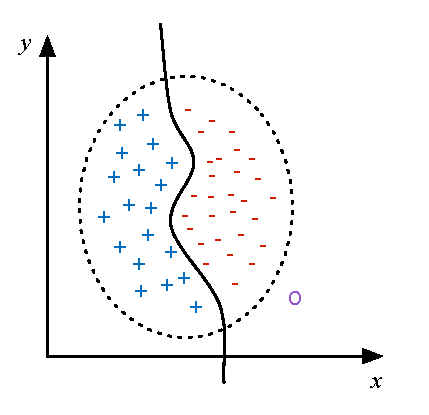
\includegraphics[width=0.5\textwidth,keepaspectratio]{./Figures/chapter3/two-vs-one-classification.pdf}
  \caption[Difference between two and one-class classification]{This plot shows the difference between two and one-class classification. The solid line indicates a possible decision boundary between the \textbf{+1} and \textbf{-1} example objects. The dashed circle indicates the closed boundary around all the data objects. In the first type the object \textbf{o} is considered to be member of the \textbf{-1}-class, whilst in the latter (\gls{occ}) formulation it is an outlier.}
  \label{fig:two-vs-one-classification}
\end{figure}

The \gls{occ} algorithms have been applied to a wide range of applications.
The first is, obviously, outlier detection of objects which do not resemble the bulk of the training data.
It can be a goal by itself and can be used as a filtering mechanism for other data processing methods.
Often methods that rely on data characteristics are sensitive for remote regions in the data set.
Using \gls{occ} these remote regions can be removed from the data set.
A second application is for the problem as described above, in which only data from a single target class is available.
When this problems originates from \eg a monitoring process, the \gls{occ} is able to recognize abnormal system states, without the need to create (or simulate) faulty states beforehand.
The final possible application given by Tax \cite{tax2001one} is the comparison of two data sets.
By constructing a \gls{occ}-classifier using a training data set, one can compare that set to a new data set.
This will result in a similarity measure expressed in the properties of outliers.
This is related to other methods of expressing similarity, such as density-ratio estimation and the \gls{kl} divergence as discussed in \Cref{sec:change_detection_time_series}.

\subsection{One-Class Classification methods}\label{subsec:occ-methods}
The methods and algorithms used for the \gls{occ}-problem can be organized into three categories \cite{tax2001one,noumir2012simple}, visually represented in \Cref{fig:occ-methods}.
The first category consists of methods that estimate the density of the training data and set a threshold on this density.
Among those are Gaussian models, \glspl{gmm} and Parzen density estimators.
In order to get good generalization results with these methods, the dimensionality of the data and the complexity of the density need to be restricted.
This can cause a large bias on the data.
When a good probability model is postulated, these methods work very well. %, since when one threshold is optimized, a minimum volume is automatically found for the given probability density model \cite{tax2001one}.

Boundary methods are based on Vapnik's principle\footnote{With a limited amount of data available, one should avoid solving a more general problem as an intermediate step to solve the original problem \cite{vapnik1998statistical}.} which imply in this case that estimating the complete data density for a \gls{occ} may be too complex, if one is only interested in the closed boundary.
Examples of methods that focus on the boundary (a direct threshold) of the training data distribution are K-centers, Nearest-neighborhood, and \gls{svdd}, or a combination of those methods \cite{hempstalk2008one}.
Especially \gls{svdd} has a strong bias towards minimal volume solutions.
These type of methods are sensitive to the scale and range of features, since they rely on a well-defined distance measure.
The number of objects that is required, is smaller than in the case of density methods.
The boundary method \gls{svdd}, constructed by Tax and which has shown good performance \cite{khan2010survey}, will be further discussed in \Cref{subsec:oc-svm-svdd}.

Reconstruction methods take a different approach.
Instead of focusing on classification of the data and thus on the discriminating features of data objects, they model the data.
This results in a compact representation of the target data and for any object a reconstruction error can be defined.
Outliers are data objects with a high error, since they are not well reconstructed by the model.
Examples of reconstruction methods are K-means, \gls{pca} and different kind of neural network implementations.

\begin{figure}
  \centering
    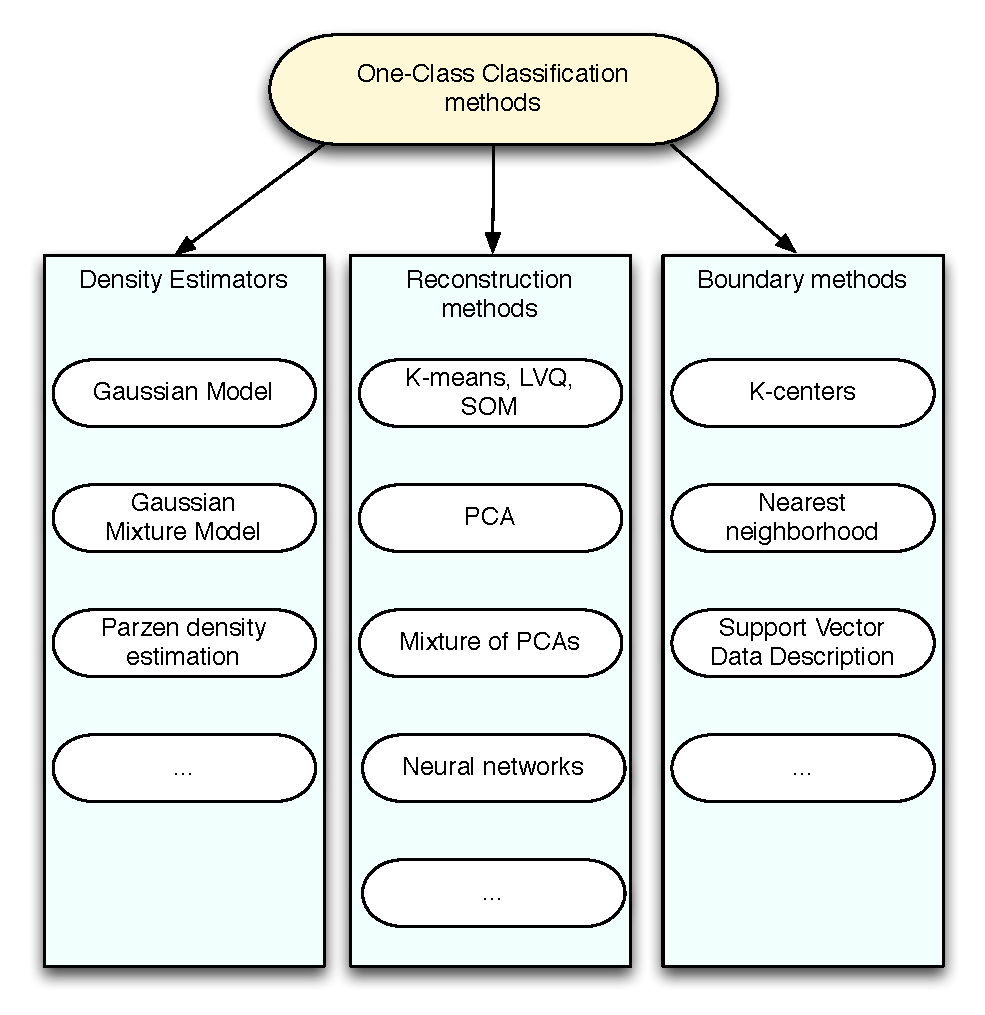
\includegraphics[width=0.5\textwidth,keepaspectratio]{./Figures/chapter3/occ_methods.pdf}
  \caption[\gls{occ} methods]{Overview of \gls{occ} methods categorized in Density Estimation, Reconstruction methods, and Boundary methods. This categorization follows the definition of Tax in \cite{tax2001one}.}
  \label{fig:occ-methods}
\end{figure}

In \cite{khan2010survey,noumir2012simple} an overview of applications for \gls{occ}-algorithms, and explictly for \gls{svm}-based methods (such as \gls{svdd} and \gls{nu-svm}), is given.
It shows succesful applications for, amonst others, problems in the field of Handwritten Digit Recognition, Face Recognition Applications, Spam Detection and Anomaly Detection \cite{li2003improving,perdisci2006using}.
As discussed in \Cref{sec:change_detection_time_series}, this can be used for change detection in time series data.

In this Section we have discussed the problem of \gls{occ} and different kind of implementations.
An often used implementation is the \gls{svm}-based method \cite{noumir2012simple}, since is shows good performance in comparitive researches \cite{khan2010survey,smola1998connection}.
In the following section (\ref{sec:one_class_svm}) two implementations of \gls{oc-svm} will be discussed, the \gls{svdd} method of Tax and Duin \cite{tax1999support} and the \gls{nu-svm}-algoritm by Sch\"olkopf.

% -- Literature --

% ``A survey of recent trends in one class classification'' \cite{khan2010survey}. 25, 2010 \\

% ``One-class classification by combining density and class probability estimation'' \cite{hempstalk2008one}. 51, 2008 \\

% ``One-class classification'' \cite{tax2001one}. 693, 2001 \\

% ``The One-Class Classification Approach to Data Description and to Models Applicability Domain'' \cite{baskin2010one}. 19, 2009 \\

% ``One-class classifier networks for target recognition applications'' \cite{moya1993one}. 70, 1993. Origin of term ``One-Class Classification'' \\
% !TEX root = ../../main.tex
\section{One-Class Support Vector Machine}\label{sec:one_class_svm}
In this section we will discuss the details of an \gls{svm} and \gls{oc-svm} implementations.
The classical implementation of an \gls{svm} is to classify a dataset in two distinct classes.
This is a common use case, although sometimes there is no training data for both classes available.
Still, one would like to classify new data points as regular, in-class, or out-of-class, \eg in the case of a novelty detection.
With that problem only data examples from one class are available and the objective is to recognize new data points that are not part of that class.
This unsupervised learning problem is closely related to density estimation.
In that context, the problem can be the following.
Assume an underlying probability distribution $P$ and a data point $\vectorsym{x}$ drawn from this distribution.
The goal is to find a subset $S$ of the input space, such that the probability that $\vectorsym{x}$ lies inside of $S$ equals some predetermined value $\nu$ between $0$ and $1$ \cite{scholkopf1999support}.

In the following of this section we will start with a discussion of traditional \glspl{svm}.
In \Cref{subsec:kernels} we will show how kernels allow for non-linear decision functions.
That is followed by two different implementations of \gls{oc-svm}: \gls{nu-svm} in \Cref{subsec:nu-svm} by Sch\"olkopf \etal \cite{scholkopf1999support}, which closely follows the above problem statement regarding density estimation, and \gls{svdd} by Tax and Duin \cite{tax1999support} in \Cref{subsec:oc-svm-svdd}.
The final part of this section discusses the influence of model parameters on the performance of \glspl{svm}

%--------------------------------------------
\subsection{Support Vector Machine}\label{subsec:svm}
We will first discuss the traditional two-class \gls{svm} before we consider the one-class variant, as introduced by Cortes and Vapnik in \cite{cortes1995support}.
Consider a labeled data set $\Omega = \{ (x_1, y_1),\allowbreak (x_2, y_2), \dots , (x_n, y_n) \}$; points $x_i \in \mathbb{I}$ in a (for instance two-dimensional) space where $x_i$ is the $i$-th input data point and $y_i \in \{-1, 1\}$ is the $i$-th output value, indicating the class membership.

An \gls{svm} can create a boundary between linear-separable data points, making it a binary linear classifier.
More flexible non-linear boundaries can be obtained by the use of a non-linear function $\phi(x)$, as illustrated in \Cref{fig:kernel_mapping}.
This function maps the input data from space $\mathcal{I}$ to a higher dimensional space $\mathcal{F}$.
The \gls{svm} can create a linear separating hyperplane in the space $\mathcal{F}$ that separates the data points from the two classes.
When the hyperplane is projected on to the (lower) original input space $\mathcal{I}$ it creates a non-linear separating curve.
A schematic overview of this process is illustrated in \Cref{fig:svm_mapping_spaces}.
The original data points $x \in \mathcal{I}$ are projected by $\phi(x)$ to the points $z \in \mathcal{F}$.
In that space the linear hyperplane is constructed by weights $w$.
This results in a non-linear hyperplane $y$ in input space $\mathcal{I}$.
The mapping and projection of data points can be efficient (and implicit) performed by using the kernel trick, which is discussed in \Cref{subsec:kernels}.

\begin{figure}
\centering
  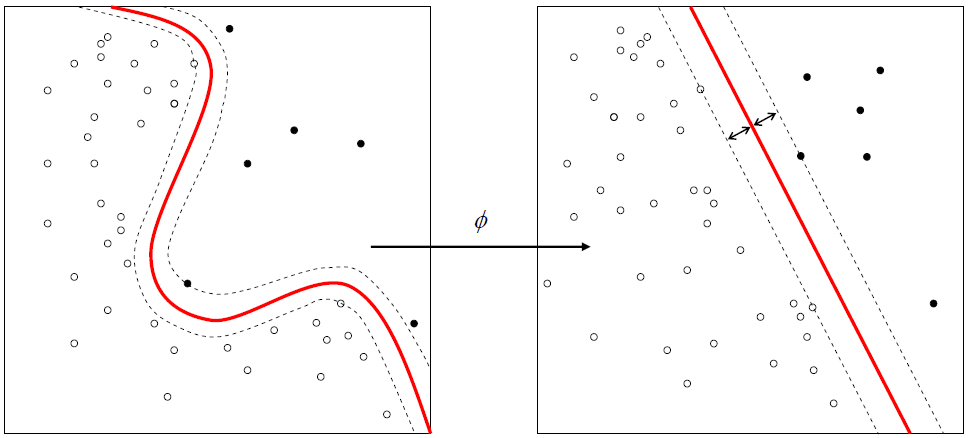
\includegraphics[width=0.8\textwidth]{./Figures/chapter3/svm_kernel_mapping.png}
  \caption[Kernel mapping]{Visualization of an \gls{svm} in 2D.
  The non-linear boundary in the input space $\mathcal{I}$ (left) is transformed to a linear boundary in the feature space $\mathcal{F}$ (right) by mapping the data points with the function $\phi$.
  The kernel trick uses a function $K$ which performs an implicit mapping. Image from Wikipedia.org}
  \label{fig:kernel_mapping}
\end{figure}

\begin{figure}
\centering
  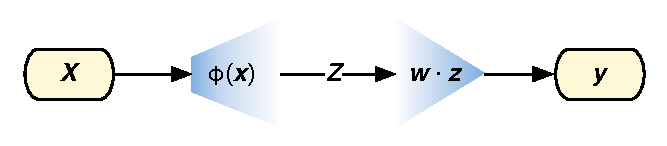
\includegraphics[width=0.8\textwidth]{./Figures/chapter3/svm_mapping_spaces.pdf}
  \caption[Mapping spaces in \gls{svm}]{Schematic visualization of the non-linear mapping of \glspl{svm}.
  The input vector $\vectorsym{x}$ from input space $\mathcal{I}$ is mapped by a non-linear function $\phi(\vectorsym{x})$ to a feature vector $\vectorsym{z}$ in the high dimensional feature space $\mathcal{F}$.
  The weights of $\vectorsym{w}$ create a linear separating hyperplane, which maps the high dimensional vector to the predicted outcome $\vectorsym{y}$.}
  \label{fig:svm_mapping_spaces}
\end{figure}

The separating hyperplane is represented by
\begin{equation}
w^T x + b = 0,
\end{equation}
with $w \in \mathcal{F}$ and $b \in \mathbb{R}$.
The hyperplane that is created determines the \emph{margin} between the classes; the minimal distance from the data points to the hyperplane.
In geometric sense, $w$ is the normal vector indicating the direction of the hyperplane and $\frac{b}{\lVert{w}\rVert}$ determines the offset of the hyperplane from the origin.
Since the size of the margin is equal to $\frac{2}{\lVert{w}\rVert}$, the maximum-margin hyperplane is found by minimizing $\lVert{w}\rVert$.
The data points which lie on the boundary of the margin are the \emph{support vectors}.
This geometrical interpretation is illustrated in \Cref{fig:svm_hyperplane}.
All data points for which $y_i = -1$ are on one side of the hyperplane and all other data points (for which $y_i = 1$) are on the other side.
The minimal distance from a data point to the hyperplane is equal for both classes.
Minimizing $\lVert{w}\rVert$ results in a \emph{maximal margin} between the two classes.
Thus, the \gls{svm} searches for a maximal separating hyperplane.

\begin{figure}
\centering
  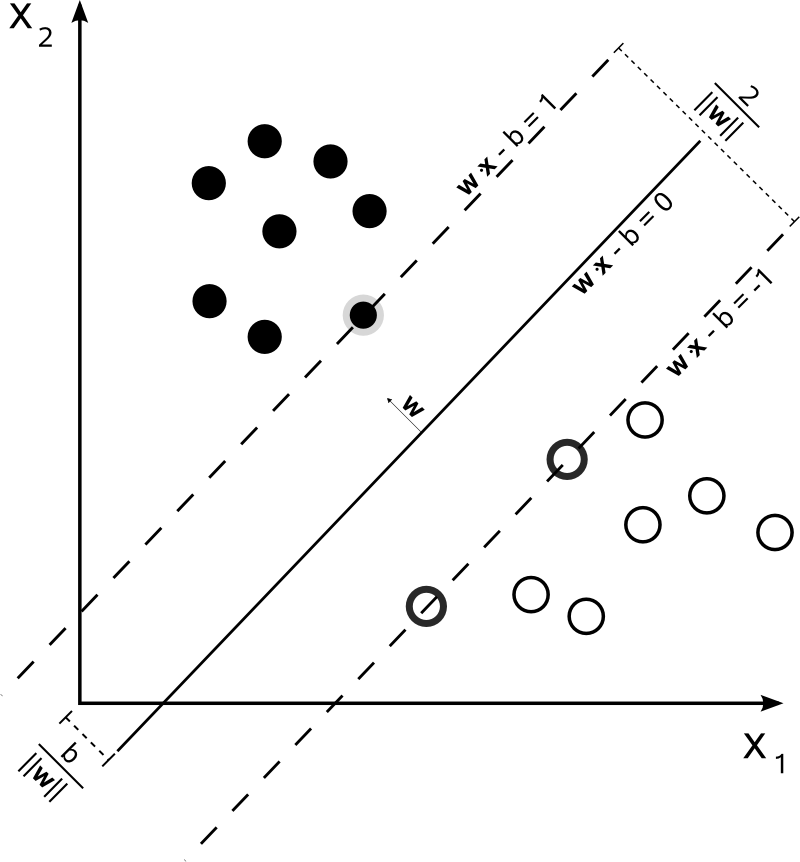
\includegraphics[width=0.5\textwidth]{./Figures/chapter3/svm_separating_plane_with_margin.png}
  \caption[\gls{svm} and the separating hyperplane]{Illustration of the separating hyperplane of an \gls{svm}.
  Here $w$ is the normal vector for the separating hyperplane and size of the margin is $\frac{2}{\lVert{w}\rVert}$.
  Image from Wikipedia.org}
  \label{fig:svm_hyperplane}
\end{figure}

With every classification method there is a risk of overfitting.
In that case the random error or noise of the data set is described instead of the underlying data.
The \gls{svm} classifier can use a \emph{soft margin} by allowing some data points to lie within the margin, instead of on the margin or farther away from the hyperplane.
For this it introduces \emph{slack variables} $\xi_i$ for each data point and the constant $C > 0$ determines the trade-off between maximizing the margin and the number of data points within that margin (and thus the training errors).
The slack variables are a generalization to minimize the \emph{sum of deviations}, rather than the \emph{number} of incorrect data points \cite{cherkassky2007learning}\footnote{if $\xi_i$ is chosen to be an indicator function, it still minimizes the \emph{number} of incorrect data points.}.
The objective function for an \gls{svm} is the following minimization function:

\begin{equation}\label{eq:svm_objective}
  \operatorname*{min}_{w,\ b,\ \xi_i} \frac{ \lVert{w}\rVert^2 }{2} + C \sum_{i=1}^n \xi_i
\end{equation}
\begin{equation}
  \begin{multlined}
  \mbox{ subject to: } \\*
  \begin{aligned}
  y_i( w^T \phi(x_i) + b) \geq \: & 1 - \xi_i & \mbox{ for all } i = 1, \dots, n \\*
   & \xi_i \geq 0 & \mbox{ for all } i = 1, \dots, n\\*
  \end{aligned}
  \end{multlined}
\end{equation}

This minimization problem can be solved (using \gls{qp}) and transformed to its (Lagrange) dual formulation.
In the dual formulation the problem scales with the number of training examples $n$ instead of the dimensionality $d$ of the samples.
Solving this problem directly in the high dimensional feature space $\mathcal{F}$ makes it intractable.
The linear approximation function corresponds to the kernel function in the dual formulation.
Solving this dual formulation is equivalent to solving the primal formulation \cite{cherkassky2007learning}.
In the dual formulation the Lagrange multipliers $a_i >= 0$ are introduced and the decision function becomes:
\begin{equation}\label{eq:svm_lagrange}
  f(x) = \operatorname{sgn}( \sum_{i=1}^n \alpha_i y_i K(x, x_i) + b),
\end{equation}
where $K(x, x_i) = \phi(x)^T\phi(x_i)$ is the dot product of data objects in feature space $\mathcal{F}$ (which is further discussed in \Cref{subsec:kernels}).
Here every data point in $\mathcal{I}$ for which $a_i > 0$ is weighted in the decision function and thus ``supports'' the classification machine: hence the name ``\acrlong{svm}''.
Since it is shown that under certain circumstances \glspl{svm} show an equality to sparse representations \cite{girosi1998equivalence,smola1998connection}, there will often be relatively few Lagrange multipliers with a non-zero value.

Using this formulation two important properties arise \cite{flach2012machine}:
\begin{enumerate}
  \item Searching for the maximum margin decision boundary is equivalent to searching for the support vectors; they are the training examples with non-zero Lagrange multipliers.
  \item The optimization problem is entirely defined by pairwise dot products between training examples: the entries of the kernel matrix $K$.
\end{enumerate}
An effect of the first property, combined with the equality to sparse representations, is that \glspl{svm} often have good results, even in the case of high dimensional data or limited training examples \cite{cherkassky2007learning}.
The second property is what enables an powerful adaptation of \glspl{svm} to learn non-linear decision boundaries.
The workings of the kernel matrix $K$ and the non-linear boundaries are discussed in the following section.

%--------------------------------------------

\subsection{Kernels}\label{subsec:kernels}
In the previous section, the mapping function $\phi(x)$ and the kernel function $K$ were briefly mentioned.
The decision function in \Cref{eq:svm_lagrange} only relies on the dot products of mapped data points in the feature space $\mathcal{F}$ (\ie all pairwise distances between the data points in that space).
It shows \cite{flach2012machine} that for any function $K$ that has the same result in feature space $\mathcal{F}$, without an explicit mapping to the higher dimension $\mathcal{F}$, the dot products can be substituted by the kernel function $K$, as introduced by Aizerman~\etal \cite{aizerman1964theoretical} and applied to \glspl{svc} by Vapnik \cite{vapnik1998statistical}:
\begin{equation}
  K(\vectorsym{x}, \vectorsym{x}') = (\vectorsym{z} \cdot \vectorsym{z}') = \phi(\vectorsym{x}) \cdot \phi(\vectorsym{x}')
\end{equation}
where vectors $\vectorsym{z}$ and $\vectorsym{z}'$ are projections of data objects $\vectorsym{x}$ and $\vectorsym{x}'$ through $\phi(\vectorsym{x})$ on the features space $\mathcal{F}$.
The dot product kernel $K$ is determined by the sum
\begin{equation}
  K(\vectorsym{x}, \vectorsym{x}') = \sum_{j=1}^m g_j(\vectorsym{x}) g_j(\vectorsym{x}')
\end{equation}
of basis functions $g_j(\vectorsym{x})$.
Note that the evaluation of dot products in the feature space $\mathcal{F}$ between vectors is performed indirectly via the evaluation of the kernel $K$ between (support) vectors in the input space $\mathcal{I}$.
This is known as the \emph{kernel trick} and gives the \gls{svm} the ability to create non-linear decision function without high computational complexity.

The kernel function $K$ can have different forms, such as linear, polynomial and sigmoidal but the most used (and flexible) form is the Gaussian \gls{rbf}.
The basis functions have the form
\begin{equation}
  g(x) = \operatorname*{sign} \left(  \sum_{i=1}^{n} \alpha_i \operatorname*{exp} \left\{ \frac{\rVert \vectorsym{x} - \vectorsym{x}_i \rVert ^2}{\sigma^2} \right\} \right),
\end{equation}
where $\sigma$ defines the width and $\rVert \vectorsym{x} - \vectorsym{x}' \rVert ^2$ is the dissimilarity measure expressed as Euclidian distance.
The inner product kernel $K$ then becomes
\begin{equation}
  K(\vectorsym{x}, \vectorsym{x}') = \operatorname*{exp} \left\{ - \frac{ \rVert \vectorsym{x} - \vectorsym{x}' \rVert ^2}{\sigma^2} \right\}.
\end{equation}
The kernel $K$ maps input space $\mathcal{I}$ to the feature space $\mathcal{F}$ which is a \gls{rkhs} of (theoretically) infinite dimensions.
As Smola \etal \cite{smola1998connection} state, this Gaussian kernel yields good performance, especially when no assumptions can be made about the data.
As an explanation, they show a correspondence between learning \glspl{svm} with \gls{rbf} kernels and good regularization operators.
This may give insights in why \glspl{svm} have been found to exhibit high generalization ability (by learning with few training objects).

The number of basis functions, the center parameters that correspond with support vectors, and the weights in the output layer are all automatically determined via the optimal hyperplane in features space $\mathcal{F}$ \cite{cherkassky2007learning}.
The width parameter $\sigma$ is equal for all basis functions and is set a priori and determines the flexibility and complexity of the boundary.
In \Cref{subsec:svm_model_parameters} this (hyper)parameter for an \gls{svm} is further discussed.

The mapping from input space $\mathcal{I}$ to $\mathcal{F}$ via $\phi(x)$ is subject to some continuity assumptions.
This general assumption in pattern recognition, states that two near objects in feature space should also resemble each other in ``real life'' \cite{tax2001one}.
Thus, objects which are close in feature space should be close in the original input space.
When this assumption does not hold, the example objects would be scatter through the feature space and finding a decision function becomes very complex.

% -- Quotes and refs to use --x

% sparsity, \gls{rkhs}: \cite{girosi1998equivalence} \\

% Use Chapter 2 from ``Learning with kernels'', \cite{scholkopf2002learning}.

%--------------------------------------------

\subsection{\acrlong{nu-svm}}\label{subsec:nu-svm}
The first of the \gls{oc-svm} methods we will discuss is often referred to as \gls{nu-svm} and introduced by Sch\"olkopf \etal \cite{scholkopf1999support}.
Instead of estimating the density function of an distribution $P$, it focuses on an easier problem: the algorithm finds regions in the input where the ``probability density lives''.
This results in a function such that most of the data is in the region where the function is nonzero.

The constructed decision function $f(x)$ resembles the function discussed in \Cref{subsec:svm}.
It returns the value $+1$ in a (possibly small) region capturing most of the data points, and $-1$ elsewhere.
The method maps the data points from input space $\mathcal{I}$ to a feature space $\mathcal{F}$ (following classical \glspl{svm}).
In that space the data points are separated from the origin by a hyperplane, with maximal margin.
Since the mapping to the feature space is based on dot products of the data points, outlier objects (which are dissimilar from the training set) will be closer to the origin.
Thus, maximizing the distance from the hyperplane to the origin increases the discriminating ability of the decision function.
Furthermore, it holds an intuitive relationship with the classical two-class \gls{svm}.

For a new data points $x$, the function value $f(x)$ determines whether the data point is part of the distribution (\ie the value is $+1$) or a novelty (\ie the value is $-1$).
The hyperplane is represented by $g(x) = w \cdot \phi(x) + \rho = 0$ and the decision function is $f(x) = \operatorname{sgn}(g(x))$.
This hyperplane and the separation from the origin is illustrated in \Cref{fig:nu-svm}.

\begin{figure}
  \centering
    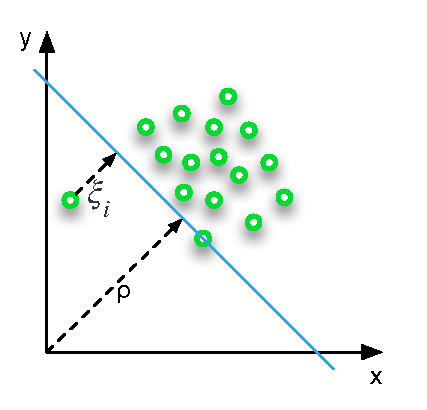
\includegraphics[width=0.5\textwidth,keepaspectratio]{./Figures/chapter3/nu-svm.pdf}
  \caption[\gls{nu-svm}]{Graphical representation of \gls{nu-svm}. The separating hyperplane $w \cdot \phi(x_i) + \rho = 0$ create a maximal margin, in the feature space, between the data points and the origin. Slack variables $\xi_i$ are used to create a soft margin.}
  \label{fig:nu-svm}
\end{figure}

The objective function to find the separating hyperplane is the following minimization function, which can be solved using \gls{qp}:

\begin{equation}\label{eq:nu-svm_objective}
  \operatorname*{min}_{w,\ \xi_i,\ \rho } \frac{\lVert w \rVert ^2}{2} + \frac{1}{\nu n} \sum_{i=1}^n \xi_i - \rho
\end{equation}
\begin{equation}
  \begin{multlined}
    \mbox{ subject to: } \\
    \begin{aligned}
      (w \cdot \phi(x_i)) \geq \: & \rho - \xi_i & \mbox{ for all } i = 1, \dots, n \\
      & \xi_i \geq 0 & \mbox{ for all } i = 1, \dots, n \\
    \end{aligned}
  \end{multlined}
\end{equation}

The decision function in the dual formulation with Lagrange multipliers is denoted as:
\begin{equation}\label{eq:nu-svm_lagrange}
f(x) = \operatorname{sgn}((w \cdot \phi(x_i)) - \rho) = \operatorname{sgn}( \sum_{i=1}^n \alpha_i K(x, x_i) - \rho)
\end{equation}

In the classical \gls{svm} objective function, as denoted in \Cref{eq:svm_objective}, the parameter $C$ decided the smoothness of the boundary, with respect to the slack variables $\xi_i$.
In the formulation of \gls{nu-svm} the equivalent parameter is $\nu \in (0,1)$ (hence the name).
It characterizes the solution in two ways:
\begin{enumerate}
  \item $\nu$ is an upper bound on the fraction of outliers, \ie training examples regarded as out-of-class.
  \item $\nu$ is a lower bound on the fraction of \glspl{sv}, \ie training examples with a nonzero Lagrange multiplier $\alpha_i$.
\end{enumerate}
When $\nu$ approaches $0$, the penalty factor for nonzero Lagrange multipliers ($\frac{1}{\nu n}$) becomes infinite, and thus the solution resembles a \emph{hard margin} boundary.

This method creates a \emph{hyperplane}, characterized by $w$ and $\rho$, that separates the data with maximal margin from the origin in the feature space $\mathcal{F}$.
In the following section we will discuss an alternative method, which uses an circumscribing \emph{hypersphere} to characterize the training data.
The region inside the hypersphere indicates the region $S$ where the probability that a data point drawn from $P$ is equal to $\nu$.


%--------------------------------------------

\subsection{\acrlong{svdd}}\label{subsec:oc-svm-svdd}
The method introduced by Tax and Duin \cite{tax1999support}, known as \acrlong{svdd}, follows a spherical instead of planar approach.
The boundary, created in feature space $\mathcal{F}$, forms a hypersphere around the (high density region of the) data.
The volume of this hypersphere is minimized to get the smallest enclosing boundary.
The chance of accepting outlier objects is thereby also minimized \cite{tax2003online}.
By allowing outliers using slacks variables, in the same manner as classical \gls{svm} and \gls{nu-svm}, a soft margin is constructed.

\begin{figure}
  \centering
    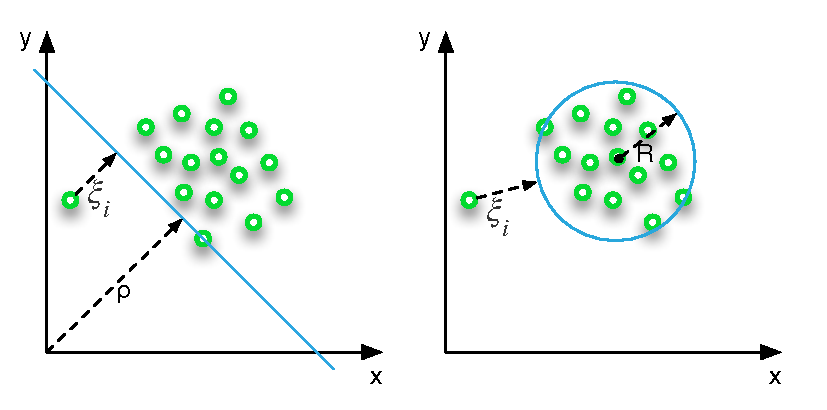
\includegraphics[width=0.8\textwidth,keepaspectratio]{./Figures/chapter3/nu-vs-svdd.pdf}
  \caption[Difference \gls{nu-svm} and \gls{svdd}]{Graphical representation of the difference between \gls{nu-svm} (left) and \gls{svdd} (right). Note that for the sake of simplicity the kernel functions are not applied.}
  \label{fig:nu-vs-svdd}
\end{figure}

The constructed hypersphere is characterized by a center $\mathbf{a}$ and a radius $R > 0$ as distance from the center to (any data point that is a \gls{sv} on) the boundary, for which the volume, and thus the radius $R$, will be minimized.
The center $\mathbf{a}$ is a linear combination of the support vectors.
Like the classical \gls{svm} and \gls{svdd} it can be required that all the distances from the data points $x_i$ to the center $\mathbf{a}$ are strict less than $R$ (or equivalent measure).
A soft margin can be allowed by using slack variables $\xi_i$.
In that case, the penalty is determined by $C$ and the minimization is expressed as \Cref{eq:svdd_objective}.
This principle is illustrated in the right image or \Cref{fig:nu-vs-svdd}.
Instead of a separating hyperplane, constructed by \gls{nu-svm} and illustrated on the left of the Figure, the \gls{svdd} creates a hypersphere (in the illustration a circle) around the data points.
By using kernel functions (\eg the \gls{rbf}) the hyperspheres in the high dimensional feature space $\mathcal{F}$ corresponds to a flexible and tight enclosing boundary in input space $\mathcal{I}$.
Possible resulting closed boundaries are illustrated in \Cref{fig:svdd-boundary}.
This enclosing boundary is obtained by minimizing the following error function $L$ which contains the volume of the hypersphere and the distance from the boundary to the outlier objects:
\begin{equation}\label{eq:svdd_objective}
  L(R, \vectorsym{a}, \vectorsym{\xi}) = R^2 + C \sum_{i=1}^n \xi_i
\end{equation}
\begin{equation}
  \begin{multlined}
    \mbox{ subject to: } \\
    \begin{aligned}
      \lVert x_i - \mathbf{a} \rVert ^ 2 \leq \: & R^2 + \xi_i & \mbox{ for all } i = 1, \dots, n \\
      & \xi_i \geq 0 & \mbox{ for all } i = 1, \dots, n \\
    \end{aligned}
  \end{multlined}
\end{equation}
In the dual Lagrangian formulation of this error function $L$ the multipliers $\vectorsym{\alpha}$ are maximized:
\begin{equation}\label{eq:svdd_lagrange}
  L = \sum_{i} \alpha_i(x_i \cdot x_i) - \sum_{i,j} \alpha_i \alpha_j(x_i \cdot x_j)
\end{equation}
\begin{equation}
  \begin{multlined}
    \mbox{ subject to: } \\
    \begin{aligned}
    0 \le \alpha_i \le C, \: \sum_{i} \alpha_i = 1
    \end{aligned}
  \end{multlined}
\end{equation}

In the maximization of \Cref{eq:svdd_lagrange} a large fraction of the multipliers $\alpha_i$ become zero and for a small fraction $\alpha_i > 0$.
This small fraction, for which $\alpha_i$ is non-zero, are called the \glspl{sv} and these objects lie on the boundary of the description.
The center of the hypersphere only depends on this small number of \glspl{sv} and the objects for which $\alpha_i = 0$ can be discarded from the solution.
Testing the membership of a (new) object $\vectorsym{z}$ is done by determining if the distance to the center $\vectorsym{a}$ of the sphere is equal or smaller to the radius $R$:
\begin{equation}\label{eq:svdd_test_object}
  \lVert \vectorsym{z} - \vectorsym{a} \rVert ^2 = (\vectorsym{z} \cdot \vectorsym{z}) - 2 \sum_{i} \alpha_i(\vectorsym{z} \cdot \vectorsym{x}_i) + \sum_{i,j}(\vectorsym{x}_i \cdot \vectorsym{x}_j) \le R^2
\end{equation}
As with \Cref{eq:svm_lagrange}, the solution of this equation only relies on dot products between the data points in $\vectorsym{x}$ and $\vectorsym{z}$.
This means that the kernel projection and trick, as discussed in \Cref{subsec:kernels}, can be applied to \gls{svdd} as well \cite{tax1999support,tax2002uniform}.

Because the Gaussian \gls{rbf} often yields good (\ie tight) boundaries, this set of kernels functions is commonly used:
\begin{equation}
  (\vectorsym{x} \cdot \vectorsym{y}) \rightarrow K(\vectorsym{x},\vectorsym{y}) = \operatorname{exp}\left(- \frac{\lVert \vectorsym{x} - \vectorsym{y} \rVert ^2}{\sigma^2}\right)
\end{equation}
Using this kernel function, the Lagrangian error function $L$ of \Cref{eq:svdd_lagrange} changes to:
\begin{equation}\label{eq:svdd_lagrange_kernel}
  L = 1 - \sum_{i} \alpha_i^2 - \sum_{i \ne j} \alpha_i \alpha_j K(x_i, x_j)
\end{equation}
Using \Cref{eq:svdd_test_object}, the following kernel formulation needs to hold for a new object $\vectorsym{z}$ to lie within the hypersphere:
\begin{equation}\label{eq:svdd_inequality}
  \sum_{i} \alpha_i K(\vectorsym{z}, x_i) \le \frac{1}{2} \left( 1 - R + \sum_{i,j} \alpha_i \alpha_j K(x_i, x_j) \right)
\end{equation}
When the Gaussian \gls{rbf} kernel is applied, and in case the data is preprocessed to have unit length (for the \gls{nu-svm} solution), the two different \gls{oc-svm} implementations \gls{nu-svm} and \gls{svdd} are shown to have identical solutions \cite{tax2002uniform,scholkopf2002learning}

\begin{figure}
  \centering
    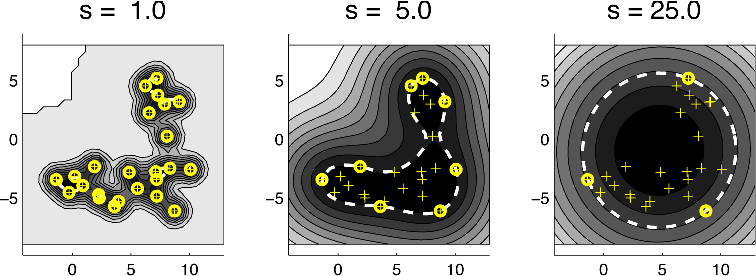
\includegraphics[width=0.5\textwidth,keepaspectratio]{./Figures/chapter3/svdd-boundary.pdf}
  \caption[\gls{svdd} boundary]{The \gls{svdd} method trained on a banana-shaped data set with different sigma-values for the \gls{rbf} kernel. Solid circles are support vectors, the dashed line is the boundary. Image by Tax \cite{tax2001one}.}
  \label{fig:svdd-boundary}
\end{figure}

%--------------------------------------------

\subsection{SVM model parameters}\label{subsec:svm_model_parameters}
\gls{svm}-model selecting and tuning depends on two type of parameters \cite{cherkassky2007learning}:
\begin{enumerate}
  \item Parameters controlling the `margin' size,
  \item Model parameterization, \eg the kernel type and complexity parameters.
  For the \gls{rbf} kernel the width parameter determines the model complexity.
\end{enumerate}

In case of a \gls{rbf} kernel, the width parameter $\sigma$ determines the flexibility and complexity of the boundary.
The value of this parameter greatly determines the outcomes of the algorithm (\eg \gls{svdd}) as illustrated in \Cref{fig:svdd-boundary}.
With a small value for the kernel width $\sigma$, each data point will tend to be used as a support vector (for almost all $\alpha_i > 0$) and the \gls{svdd} solution resembles a Parzen density estimation.
For large values of $\sigma$, the solution will resemble the original hypersphere solution (in contrast with a tight boundary around the data).
With a large value for the width $\sigma$, the boundary approximates the spherical boundary.
The influence of the $\sigma$ parameter on the \gls{svdd} solution is illustrated in \Cref{fig:svdd-boundary-sigma}.

\begin{figure}
  \centering
    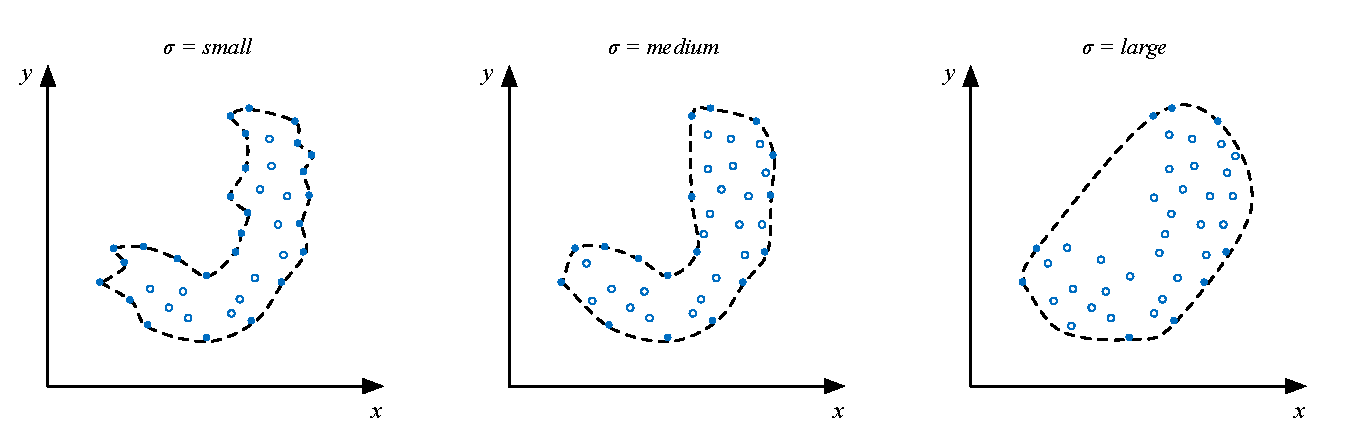
\includegraphics[width=0.8\textwidth,keepaspectratio]{./Figures/chapter3/svdd-parameter-sigma.pdf}
  \caption[\gls{svdd} boundary]{The \gls{svdd} method trained on a banana-shaped data set with different $\sigma$-values for the \gls{rbf} kernel. Solid circles are support vectors, the dashed line is the boundary.}
  \label{fig:svdd-boundary-sigma}
\end{figure}

As discussed in \Cref{subsec:nu-svm}, the \gls{svm} parameter $C$ (or $\nu$ in case of \gls{nu-svm}) is of high influence on the ``smoothness'' of the decision function.
It acts as an upper bound to the fraction of outliers and as a lower bound to the fraction of \glspl{sv}.
A more detailed discussion of the influence of the \gls{svm} model parameters can be found in Section~9.8 of \cite{cherkassky2007learning} and Section~7.4 from \cite{flach2012machine}.
A detailed discussion of the $\nu$ and kernel parameters can be found in \cite{scholkopf2002learning}.

The following chapter will discuss our proposed method, which incorporates the \gls{svdd} algorithm.
It relates the \gls{oc-svm} model construction to outlier detection and eventually change detection, leading to finding a temporal segmentation of time series data.

% -- Notes --
% \begin{itemize}
  % \item Low target rejection rate $f_{T-}$ and low outlier acceptance rate $f_{O+}$. When only target examples are present, the first one can be estimated by the number of support vectors that we obtain as a solution of Lagrangian~\ref{eq:svdd_lagrange_kernel}.
% \end{itemize}

% -- Literature --


% ``A geometric approach to support vector machine (SVM) classification'' \cite{mavroforakis2006geometric}. 136, 2006 \\

% ``Least squares one-class support vector machine'' \cite{choi2009least}. 27, 2009 \\

% ``On simple one-class classification methods'' \cite{noumir2012simple}. 2012  --> decouples radius and center optimization, gives fast approximations instead of precise results. \\

% ``Choosing a small width of the kernels leads to high generalization error as it effectively decouples the separate basis functions of the kernel expansion into very localized functions which is equivalent to memorizing the data, whereas a wide kernel tends to oversmooth.'' \cite{smola1998connection}. \\

% ``For small values of $\sigma$ almost all $\alpha_i >0$ and the \gls{svdd} resembles a Parzen density estimation.'' \cite{tax2002uniform} page 4, \cite{tax1999support} page 4. \\
% !TEX root = ../main.tex
% Chapter 4

\chapter{Application to Human Activity Time Series Data}

\label{Chapter4} % For referencing the chapter elsewhere, use~\ref{Chapter4}

\lhead{Chapter 4. \emph{Application to Human Activity Time Series Data}} % This is for the header on each page - perhaps a shortened title

%----------------------------------------------------------------------------------------

Ideen naam methode:
\begin{itemize}
  \item Human Activity Support Vector Change Detection
  \item Inertial Sensor Time Series Svm Temporal Segmentation
  \item Support Vector bases Human Activity Temporal Segmentation
  \item Human Activity Temporal Segmentation by Support Vector Machines: HATS-SVM
  \item HATS with One-Class SVM: HATS-OCS, HATS-OS, HATSOS
  \item OCS-HATS
  \item HATS-SVDD
\end{itemize}

\section{Experiment notes}
\begin{itemize}
  \item ICSS/CUSUM is goed in het vinden van variance changes. Niet goed in mean veranderingen.
  \item geprobeerd direct model-reset te doen na change point, maar dan kan je achteraf niet meer verder analyseren.
\end{itemize}


\begin{description}
  \item[Data gathering] Explain data gathering methods. Refer to chapter 5 and 6 for articifial and real-world details.
  \item[Model construction] Explain SVDD model construction and updating.
  \item[Model properties] Explain the SVDD properties that are used to calculate the change indication.
  \item[Change detection] Explain the interpretation of the properties, the possible (modulair) methods to give change indication
\end{description}


\TODO{Write chapter introduction/outline. Give overview of method approach and refer to each section for details of that stage.}

\TODO{Puts emphasis on two-stage framework by Takeuchi and Yamanishi \cite{takeuchi2006unifying}.}.

\TODO{Put somewhere difference and emphasis of online vs. offline/batch/post-processing}

\begin{figure}
  \centering
    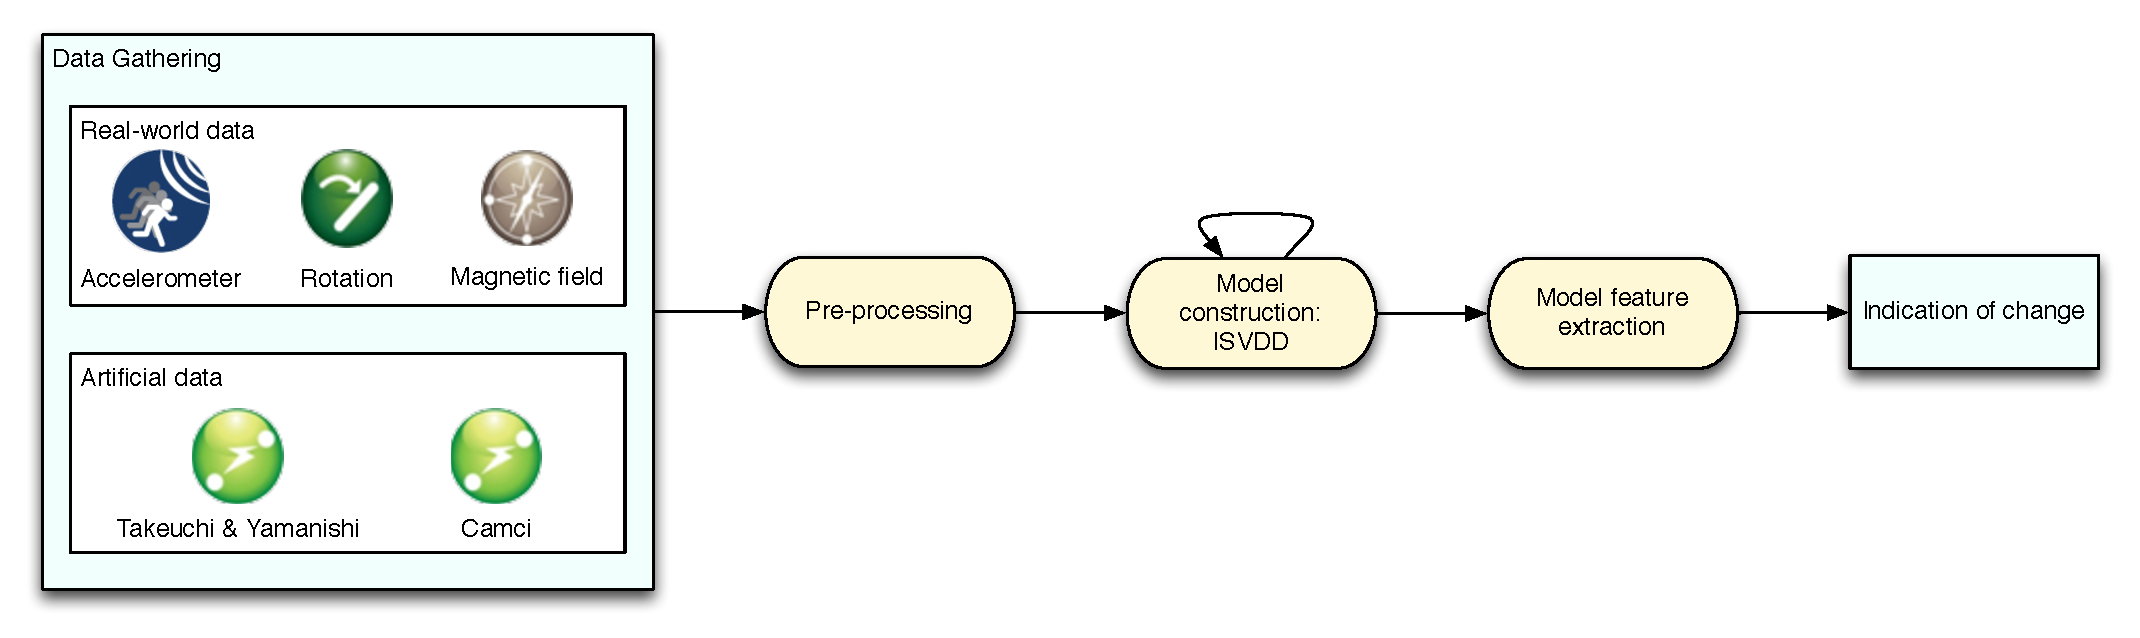
\includegraphics[width=\textwidth,height=\textheight,keepaspectratio]{./Figures/chapter4/method_setup_short.pdf}
  \caption[Method setup]{Schematic overview of the change detection method. The first step is the data gathering, described in Section \ref{sec:method_data_gathering}. Ater the pre-processing, the data is used to construct a \gls{svdd} model, as described in Section \ref{sec:method_model_construction}. Section \ref{sec:method_model_features} describes which features of the model are used for the final change indication algorithm, discussed in Section \ref{sec:method_change_detection}.}
  \label{fig:method_overview_short}
\end{figure}

% !TEX root = ../../main.tex
\section{Data Gathering}\label{sec:method_data_gathering}
In this section we briefly discuss the different data gathering methods used for the change detection algorithms and experiments.
\Cref{subsec:data_gathering_artificial} discusses the artificial data sets we will use.
In \Cref{subsec:data_gathering_real_world} an overview of the real-world data sets used is provided.
Both sections refer to Chapters~\ref{Chapter5} and~\ref{Chapter6} for more details, respectively.

% ------
\subsection{Artificial data}\label{subsec:data_gathering_artificial}
In order to provide an objective comparison to other methods, we will use artificial data sets which are also used in the earlier work on which \gls{ocs-hats} is based.
These are the data sets used by Takeuchi and Yamanishi \cite{takeuchi2006unifying} and Camci \cite{camci2010change}.
Both construct a collection of one-dimensional time series data according to a second order \gls{ar} model:
\begin{equation}
  x_t = a_1 x_{t-1} + a_2 x_{t-2} + \epsilon_t.
\end{equation}
Over the different data series the mean and variance of the Gaussian random variable $\epsilon_t$ differs and changes at pre-determined change points.
Using this data set an objective quality measure over the change detection methods can be obtained and compared.
All the used data sets are listed and analyzed in \Cref{Chapter5}.

% ------
\subsection{Real-world data}\label{subsec:data_gathering_real_world}
In the second type of data sets we apply our method for change detection and temporal segmentation to real-world data sets.
For our setup we record the activities of humans performed both in- and outdoor in an unknown environment.
Activities performed include sitting, standing, walking, running in a straight and curved line, and walking up- and downstairs.
\gls{ocs-hats} uses the signals from the accelerometer, magnetic field, and rotation sensors.
These time series data are used to detect change points.
A video recording from the performed activity is used to annotate the time series with real change points.
The discovered change points are compared with these annotated change points to give a subjective quality measure.
In \Cref{Chapter6} we give a detailed analysis of the performed activities and the recorded data sets.

For the experiments we used a smartphone with inertial sensors as recording device.
The activities were recorded using a free \textsc{Android} application \cite{sensorlogger}.
This application was chosen for its convenient data format of the sensor recording and its regularity of the sampling interval.
Table~\ref{tab:recorded_metrics} lists all the recorded metrics.
For our experiments we used the data for the accelerometer, magnetic field and rotation.

We implemented our algorithm in \textsc{Matlab}.
For the \gls{svdd} model construction phase we used the \textsc{dd\_tools} library by Tax \cite{Ddtools2013}, which depends on the \textsc{PR\_tools} package, originating from the book by Van Der Heijden \etal \cite{van2005classification}.
Alternatively, the widely used \textsc{LibSVM} \cite{chang2011libsvm} add-on for the \gls{svdd} algorithm by Chang \etal \cite{changrevisit} can be used.

\begin{center}\begin{table}
  \caption[Measured metrics]{Measured sensor metrics. The set of axis is always the triple (x, y, z) direction.}
  \begin{tabulary}{\textwidth}{|l|L|c|c|}
    \hline
    Sensor metric & Description & Units of measure & Typical range \\
    \hline \hline
    Accelerometer & Acceleration force along each axis (including gravity). & $m/s^2$ & $-20$ -- $20$ \\
    \hline
    Gravity & Force of gravity along each axis. & $m/s^2$ & $-10$ -- $10$\\
    \hline
    Gyroscope & Rate of rotation around each axis. & $rad/s$ & $-15$ -- $15$\\
    \hline
    Light & Light sensitive sensor at the front of the phone. & & $0$ -- $10000$ \\
    \hline
    Linear acceleration & Acceleration force along each axis (excluding gravity). & $m/s^2$ & $-20$ -- $20$ \\
    \hline
    Magnetic field & Geomagnetic field strength along each axis. & $\mu T$ & $-60$ -- $60$ \\
    \hline
    Orientation & Degrees of rotation around the three physical axis. & Degrees & $-100$ -- $360$ \\
    \hline
    Rotation & Measure of rotation around the device's rotation axis. & Unitless & $-1$ -- $1$\\
    \hline
  \end{tabulary}

  \label{tab:recorded_metrics}
\end{table}\end{center}

% !TEX root = ../../main.tex
\section{Model Construction: Incremental SVDD}\label{sec:method_model_construction}
After the data is collected and pre-processed (or in the case of the artificial data sets: generated), we construct an online incremental sliding window model construction algorithm.
We follow the method and implementation introduced by Tax and Laskov \cite{tax2003online}, the \acrlong{isvdd} method.
This method combines the techniques of online, unsupervised and incremental learning methods with the earlier introduced \gls{oc-svm} algorithm \gls{svdd}.
The method is first initialized with a window length and then in every step a new data object is added to and the last data object is removed from the working set.

Using the following abstract form of the \gls{svm} optimization problem, the extension of the incremental \gls{svm} to the \gls{svdd} can be carried out:
\begin{equation}
  \operatorname*{max}_\mu \operatorname*{min}_{\substack{
    0 \le x \le C \\
    \vectorsym{a}^T \vectorsym{x} + b = 0}
  } : W = -\vectorsym{c}^T\vectorsym{x} + \frac{1}{2}\vectorsym{x}^T K\vectorsym{x} + \mu(\vectorsym{a}^T\vectorsym{x} + b),
\end{equation}
where $\vectorsym{c}$ and $\vectorsym{a}$ are $n \times 1$ vectors, $K$ is a $n \times n$ matrix and $b$ is a scalar.
The \gls{svdd} implementation of this abstract form is set by the parameters $\vectorsym{c}=\operatorname*{diag}(K)$, $\vectorsym{a} = \vectorsym{y}$ and $b=1$.
The procedure for the incremental version has two operations: adding and removing a data object $k$.
When a data object $k$ added, its weight $x_k$ is initially set to $0$.
In case of an object removal, the weight is forced to be $x_k=0$.
Both the operations conclude with the recalculation $\mu$ and the weights $\vectorsym{x}$ for all the objects, in order to obtain the optimal solution for the enlarged or reduced data set.
The incremental learning algorithm follows from these two operations: new data objects are added to and old data objects are removed from the working set.

The size of the initial window of data objects has a lower bound determined by the hyperparameter $C$ (Equation \ref{eq:svdd_objective}).
Because of the equality constraint $\sum_{i=1}^n a_i x_i = 1$ and the box constraint $0 \le x_i \le C$, the number of objects in the working set must be at least $\ceil{\frac{1}{C}}$.
Thus the algorithm is initialized by selection the first $\ceil{\frac{1}{C}}$ objects for the working set.
In every step of the loop of the algorithm at least the same number of objects must be added as there are removed.
By analyzing the \gls{kkt} conditions, \cite{tax2003online} shows the optimality of the algorithm.

From experiments it shows that the online, \gls{isvdd}, method results in less false alarms than the static \gls{svdd}.
An explanation for this is that \gls{isvdd} follows the changing data distribution, such that small changes over time, like a drift in mean or increase in frequency, continuously re-model the \gls{svm} representation.
% !TEX root = ../../main.tex
\section{Model Features}\label{sec:method_model_features}
In the previous section we have discussed the \gls{isvdd} method, which creates a \gls{oc-svm} representation of a working set of data objects at every step of the algorithms loop.
This section shows how we interpret the constructed model and extract features to obtain a measure which can be used for an indication of change points.
The next section discusses how this obtained measure is used to indicate change.

The \gls{isvdd} algorithm creates a spherical \gls{oc-svm} representation of the working set at every step of the algorithm.
This model is obtained by the minimization of \Cref{eq:svdd_objective}, which incorporates the radius $R$ of the sphere and the distances $\vectorsym{\xi}$ from the outliers to the boundary.
We will use the radius $R$ of the hypersphere as an indication of change.

In \cite{tax2002uniform} Tax and Duin provide an analysis of the error of the \gls{svdd} algorithm.
This error is based on
\begin{inparaenum}[\itshape 1\upshape)]
\item the fraction $f_{T-}$ of target objects that is rejected, and
\item the fraction $f_{O+}$ of outliers that is accepted.
\end{inparaenum}
Since in \gls{occ} situations typically there are (almost) no examples of outlier objects, Tax and Duin construct a method to generate outliers based on the assumption that the the location of (potential) outliers are uniformly distributed around the target set.
To minimize the error, calculated by the fractions $f_{T-}$ and $f_{O+}$, we should minimize the volume of the target data description (\ie the boundary of \gls{svdd}).
That is because the fraction of accepted outliers $f_{O+}$ is an estimate of the volume of the target data description, with respect to the volume of the outlier distribution.
Tax and Duin provide a method to optimize the parameters of the \gls{svdd} method, \ie the trade-off parameter $C$ and the \gls{rbf} kernel width $\sigma$.
This optimization will result in the modification of the radius $R$ of \Cref{eq:svdd_objective} and affects the Lagrangian inequality~(\ref{eq:svdd_inequality}).

\begin{figure}
  \centering
    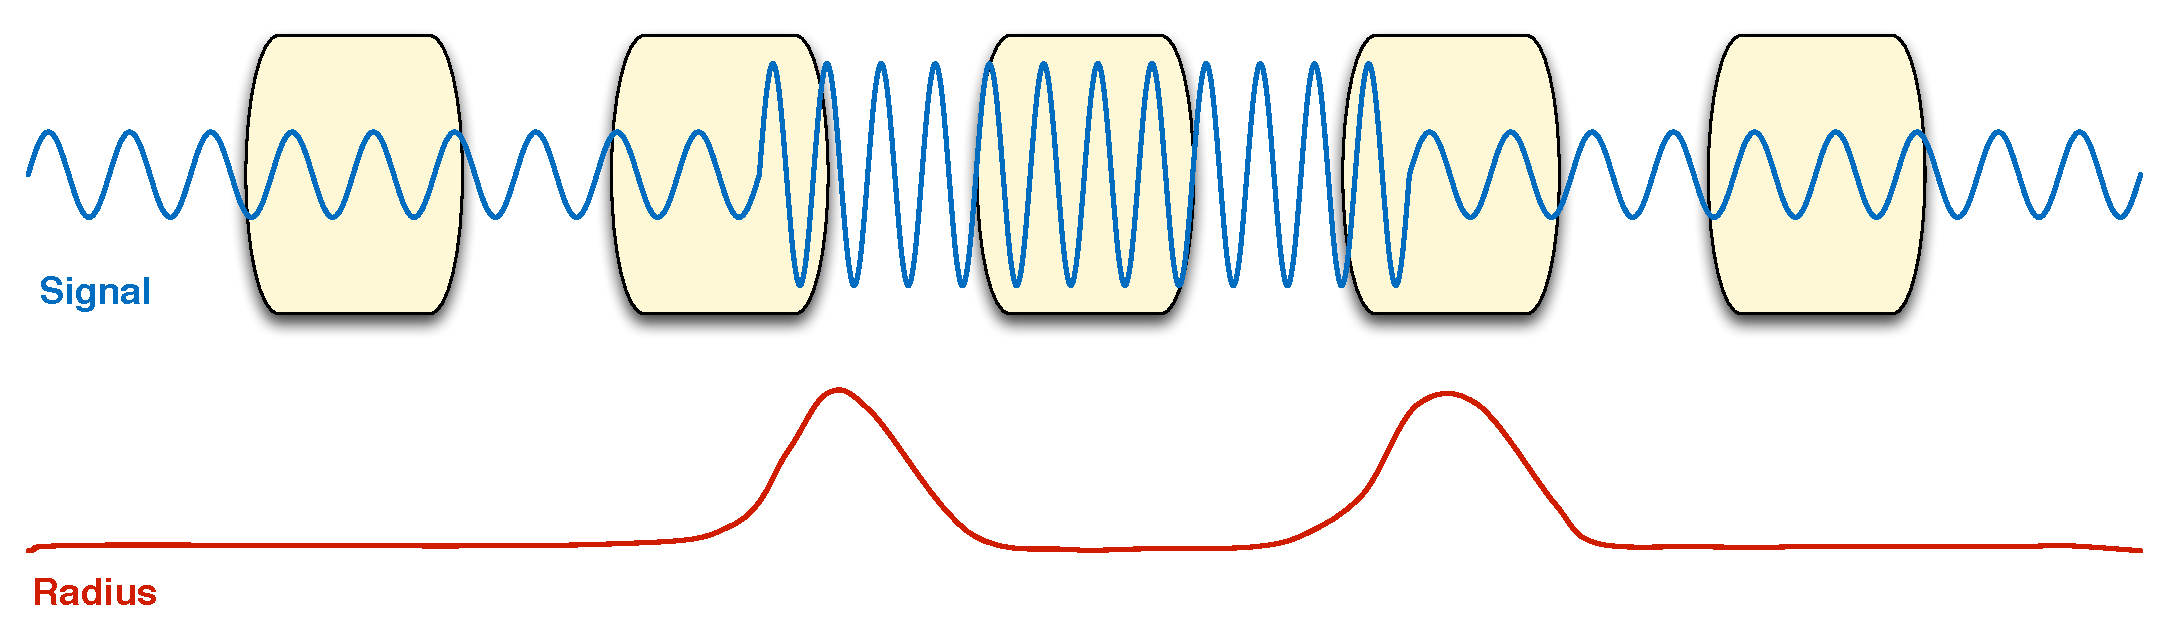
\includegraphics[width=\textwidth,height=\textheight,keepaspectratio]{./Figures/chapter4/expected_behaviour.pdf}
  \caption[Expected radius behavior]{Expected behavior of the radius $R$ of the hypersphere. The upper part shows a typical sinusoidal time series signal. The lower graph visualizes an abstract expectation of the values of $R$. Five possible time windows are illustrated. Windows $a$, $c$ and $e$ cover an area of homogeneous signal. The expected value of $R$ is low. The other two windows, $b$ and $d$ cover a change entering and leaving the window, respectively. At these locations the radius $R$ is expected to increase temporarily.}
  \label{fig:radius_expectation}
\end{figure}

Since in our method the parameters $C$ and $\sigma$ are kept constant, and thereby also the fraction of target objects being rejected, the only free parameter is the radius $R$.
During the \gls{isvdd} algorithm the volume of the hypersphere is minimized.
This means that only the radius of the sphere will change during the analysis over the time series data.
We will interpret changes in the radius $R$ with the same continuity assumptions as mentioned in \Cref{subsec:kernels}.

For instance, consider two hyperspheres that model two different, but partially overlapping, working sets of objects.
If the radius size of these two hyperspheres are close to each other, that means the distribution of objects in the sets are also similar.
In other words, if the distribution over objects in a working set changes, so does the characteristics of the set, and the radius $R$ of the hypersphere will also change.
If in the case of a change in distribution the data objects in the working set become more heterogeneous, the radius of the hypersphere will increase.
When, instead, the data objects change from a heterogeneous set to a more homogeneous, we expect the radius to decrease in value, since the data objects are closer to each other in the feature space.
This relation between the signal and expected radius $R$ is illustrated in \Cref{fig:radius_expectation}.
It shows that in the two time windows that cover a heterogeneous set of data objects, the radius of the hypersphere is expected to be relatively high.

With the \gls{isvdd} algorithm we have effectively implemented a form of dimensionality reduction by feature extraction, using the radius $R$.
The following section discusses the algorithms which can be applied to the extracted radius $R$ as a volume estimate.
We thereby follow the setup of the unifying framework by Takeuchi and Yamanishi~\cite{takeuchi2006unifying}, of which this section described the first stage.
% !TEX root = ../../main.tex
\section{Change Detection}\label{sec:method_change_detection}

 % --- OLD ---
% % !TEX root = ../../main.tex
\section{Change Indication}\label{sec:method_change_indication}
*** TODO: change section title ***
*** TODO: ***
\emph{Follow methodology of ``A unifying framework for detecting outliers and change points from time series'' \cite{takeuchi2006unifying}.
It creates a two-stage process of first searching for outliers, and then using the ``outlier-score'' to find (sudden) change points, by a weighted average of a moving window.
That eventual score can be thresholded (as in the paper) or processed with something like CUSUM (proposal).
Looks like my proposed methods, in that is combines outliers and gives a score to change points.}

The proposed method of this thesis follows the unifying framework as introduced by Takeuchi and Yamanishi \cite{takeuchi2006unifying} and an similar implementation by Camci \cite{camci2010change} with \glspl{svm}.
The unifying framework combines the detection of outliers with change points and divides it in two stages.
The first stage determines the outliers in a time series by giving a score based on the deviation from a learned model, and thereby creates a new time series.
The second stage runs on that new created time series and calculates a average over a window of the outlier scores.
The problem of change detection is then reduced to outlier detection over that average-scored time series.
This method is named \gls{changeFinder} by the authors.
The implementation by Camci, which uses \glspl{svm} to detect changes is named \acrlong{svcpd}.

The problem statement and formal definition, following Tackeuchi and Yamanishi \cite{takeuchi2006unifying} and Camci \cite{camci2010change} is the following.
The algorithm needs to find \emph{sudden} changes in the time series data.
In other words, slowly changing properties in the data are not considered to be changes.
This is in line with the search of changes in activities, since we are only interested in different activities (which are represented by sudden changes) instead of changes within an activity.
Considered a time series $x_1 x_1 \dots$, which is drawn from a stochastic process $p$.
Each $x_t$ (t = 1, 2, \dots) is a $d$-dimensional real valued vector and $p$ a probability density function of the sequence $x_1 x_2 \dots$.
Assume $p$ can be decomposed in two different \gls{iid} stationary stochastic processes $p^1$ and $p^2$ and are one-dimensional Gaussian density functions.
For a time point $a$ data points for which $t < a$ are drawn from $p^1 = N(\mu_1, \sigma_1^2)$ and for $t \geq a$ from $p^2 = N(\mu_2, \sigma_a^2)$.
If $p^1$ and $p^2$ are different, then the time point $t = a$ is a \emph{change point}.
In \cite{takeuchi2006unifying} the similarity between the stochastic processes are expressed by the \gls{kliep} divergence $D(p^2||p^1)$.
The problem with this measure is that, as the authors conclude and Camci discusses, it is not able to detect a change by decrease in variance.

Whereas \gls{changeFinder} uses double probability estimation algorithm, our approach follows \gls{svcpd} by constructing a \gls{svm} over a sliding window.
The \gls{svcpd} algorithm uses the location of new data points in the feature space $\mathcal{F}$ with respect to the hypersphere and the hypersphere's radius $R$ to determine whether the new data point represents a change point.

*** TODO: What is my contribution compared to Camci? Distance of outliers to hypersphere? ***
% % !TEX root = ../../main.tex
\section{Overview}\label{sec:method_overview}

\begin{figure}
  \centering
    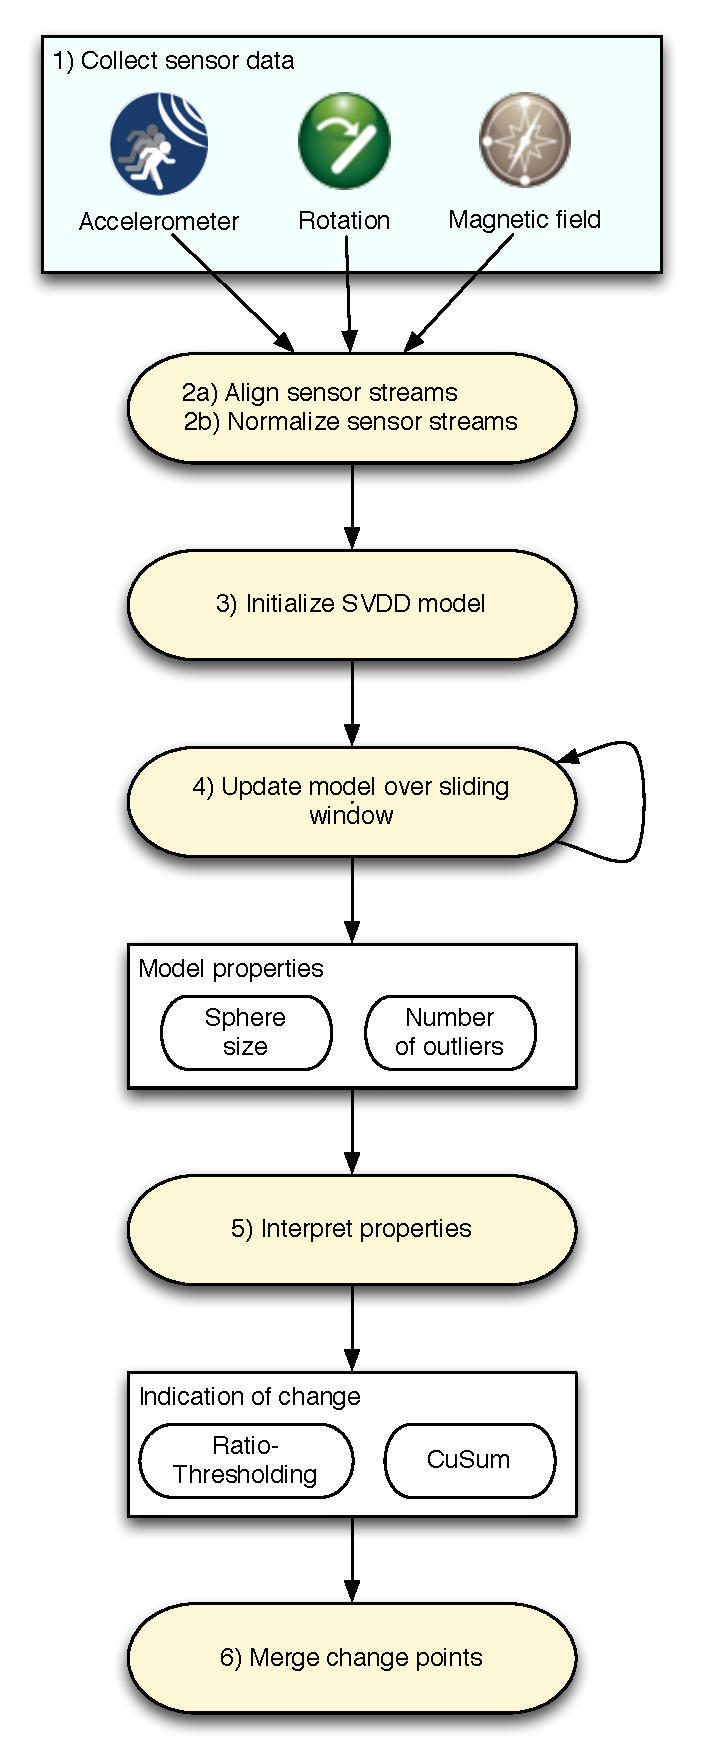
\includegraphics[width=\textwidth,height=\textheight,keepaspectratio]{./Figures/graphs/chapter4/method_setup.pdf}
  \caption[Method setup]{Schematic representation of the change detection method.}
  \label{fig:method_overview}
\end{figure}

This section gives a description of the method used for the experiments and change detection mechanism.
First described is the method to process the gathered sensor data.
A schematic overview is given in figure \ref{fig:method_overview} and shows the steps of the method.
A more detailed explanation of the ``Update model'' step follows.
This section is finalized with the experiments setup, annotation of data streams and quality measure.

\subsection{Change detection method}
As graphically represented in figure \ref{fig:method_overview}, the change detection method starts by processing the data from sensor, such as the accelerometer, magnetic orientation and rotation measures \footnote{Something about the origin of the streams; all from the same sensor or different sensors?}.

The first step is to process the raw streams of data originating from a multiple of sensors.
The two processes applied are alignment and normalization.
Due to noisy sampling, not all the timestamps in the data streams are sensed at the same timestamp.
Since the \gls{svdd} method requires all the data stream at every timestamp and can not handle missing data on one of the timestamps, all the unique timestamps are filtered out.
Whilst this results in an overall filtering effect, in practice between $1\%$ and $5\%$ of each data stream is disregarded.
The effect of this filtering is not significant and the data is not modified.

Due to the nature of the sensor signals, a normalization step is required in order to set the weight for all the data streams equal.
The range of the accelerometer signal typically spans $-20$ to $20$, the magnetic field from $-60$ to $60$ and the rotations range is from $-1$ to $1$.
This means that a relative small change in the accelerometer stream could have a much larger impact on the model than the same (absolute) change in the rotation stream, whilst the latter has a larger relative impact.
The normalization step ensures that all data is weighted equally and changes in the data are all proportional.

In step $3$ the \gls{svdd} model is initialized.
The first full window over the data stream is used to construct an initial model.
During the initialization the parameters for the \gls{svdd} are provided, begin the kernel type (radial), \gls{rbf} with $\sigma$ and the outlier-fraction $C$.

Step $4$ is executed for every step-size $s$ data points in the stream.
Every update the oldest $s$ data points are removed from and $s$ new data points are added to the \gls{svdd} model.
The model is (partially) reconstructed and new model properties, such as the radius of the hypersphere and the number of outliers, are the result of this step \footnote{Other measures are also possible, for instance the distance from all the outliers to the boundary of the hypersphere}.
*** MORE ON THE UPDATING STEP ***

This final step of this method, step $5$, is the interpretation of the model properties.
Many algorithms can be used for this process, all which take a one-dimensional time series as input and determine where change has occured.
In our setup we used the \gls{rt} and \gls{cusum} methods, to show the modularity of this step.

\subsection{Model updating}

\subsection{Experiments}
For the experiments we used a HTC Sensation XE smartphone as recording device.
The activities were recorded using a free Android application \cite{sensorlogger}.
This application was chosen for its convenient data format of the sensor recording and its regularity of the sampling interval.
Table \ref{tab:recorded_metrics} lists the recorded metrics.
For our expiments we used the data for the accelerometer, magnatief field and rotation.

\begin{center}\begin{table}
  \begin{tabulary}{\textwidth}{|l|L|c|c|}
    \hline
    Metric & Description & Units of measure & Typical range \\
    \hline \hline
    Accelerometer & Acceleration force along each axis. & $m/s^2$ & $-20$ -- $20$ \\
    \hline
    Gravity & Force of gravity along each axi.s & $m/s^2$ & $-10$ -- $10$\\
    \hline
    Gyroscope & & $rad/s$ & $-15$ -- $15$\\
    \hline
    Light & Light sensitive sensor at the front of the phone. & & $0$ -- $10000$ \\
    \hline
    Linear acceleration & & $m/s^2$ & $-20$ -- $20$ \\
    \hline
    Magnetic field & Geomagnetic field strength along each axis. & $\mu T$ & $-60$ -- $60$ \\
    \hline
    Orientation & & & $-100$ -- $360$ \\
    \hline
    Rotation & & & $-1$ -- $1$\\
    \hline
  \end{tabulary}
  \caption{Measured metrics. The set of axis is always the triple (x, y, z) direction.}
  \label{tab:recorded_metrics}
\end{table}\end{center}


% !TEX root = ../main.tex
% Chapter 5

\chapter{Artificial data results}

\label{Chapter5} % For referencing the chapter elsewhere, use~\ref{Chapter5}

\lhead{Chapter 5. \emph{Artificial data results}} % This is for the header on each page - perhaps a shortened title

%----------------------------------------------------------------------------------------
\section{Outline}
\emph{Not intented for the reader.}
\begin{itemize}
  \item Compare proposed method with methods of Chapter~\ref{Chapter2}
  \item Provide KL-analysis (as Takeuchi does)
  \item Provide plots, tables, graphs, error rates, precision, etc.
  \item Apply to a multiple of data, to compare to previous research - use that data
  \item Give theoretical analysis about performance. Big-O, memory, run-time, precision.
  \item This sections needs programmed implementations of own method and the ones compared
\end{itemize}

% % !TEX root = ../../main.tex
\section{Artificial Data}\label{sec:artificial_data}
\TODO{Use data from \cite{camci2010change,takeuchi2006unifying}}
In this section we present three data sets as used by \cite{camci2010change,takeuchi2006unifying} to provide for a objetive performance comparison.
% % !TEX root = ../../main.tex
\section{Real-world Data}\label{sec:real_world_data}

% Chapter 6

\chapter{Conclusions} % Main chapter title

\label{Chapter6} % For referencing the chapter elsewhere, use \ref{Chapter1} 

\lhead{Chapter 6. \emph{Conclusions}} % This is for the header on each page - 
%perhaps a shortened title

%----------------------------------------------------------------------------------------

\section{}
% !TEX root = ../main.tex
% Chapter 7

\chapter{Conclusion}

\label{Chapter7} % For referencing the chapter elsewhere, use~\ref{Chapter7}

\lhead{Chapter 7. \emph{Conclusion}} % This is for the header on each page - perhaps a shortened title

%----------------------------------------------------------------------------------------
\section{Outline}
\emph{Not intended for the reader.}
\begin{itemize}
  \item Tie together, integrate, synthesize all the issues from the chapters, reflecting on introductory thesis statements.
  \item Provide answers to research questions
  \item Highlight study limitations
  \item Directions for further research.
  \item Content: Summarize
  \begin{itemize}
    \item What have I researched
    \item Main arguments
    \item How researched
    \item What discovered
    \item What pre-existing views were challenged (?)
  \end{itemize}
  \item Overview of
  \begin{itemize}
    \item New knowledge
    \item Significance of research
    \item Limitations (data, concepts)
    \item Speculations on implications of research
    \item Further research and development, or: links with different fields, other methods applied to same data.
  \end{itemize}
  \item Must: make clear statement of my original contribution
  \item Ideally:
  \begin{itemize}
    \item Shows links across key ideas spread in chapters
    \item Show commitment and enthusiasm for research
    \item Positive impression
  \end{itemize}
  \item Avoid:
  \begin{itemize}
    \item claim findings that have not been proven
    \item introducing new data/concepts
    \item Be self-critical, but dont put weaknesses or limitation in research
    \item Too long/too short
  \end{itemize}
\end{itemize}


Paragraph: into on conclusion; what have I researched and what is my contribution.
Break into sections further down.

===

In this research we have applied \gls{occ} methods to accelerometer data, recorded during the performance of various human activities, in order to create a temporal segmentation of those recordings.
The goal was to find the change points between activities, assuming that it will aid better understanding of the sensor values.
To do so, we used the \gls{svdd} algorithm by Tax~\cite{tax1999support}, following the method of applying it to a sliding window of data, as done by Camci~\cite{camci2010change}.
Instead of using both the information whether a new data point is an outlier and the radius of the hypersphere to indicate change, we only used on the latter model properties.
The increase of the radius of the constructed hypersphere, which encloses the data objects and increases with heterogeneous segments of data, is extracted and used for indication of change.

\TODO{Write overview of this chapter. \emph{In the following section we will...}}


\section{What is done}
The scope of this research was the temporal segmentation of recordings, obtained from human activities.
This was performed in the wider context of activity classification.
Currently, many algorithms obtain an implicit segmentation as a side-effect of direct activity classification.
In this research the primary goal was finding a temporal segmentation, which is assumed to be able to aid the classification step.

We have considered a range of segmentation methods, from which the method by Camci~\cite{camci2010change} showed potential.
It is based on the detection of outliers in a time series data, assuming that an increase of outliers indicates a change in the underlying generating model.
For the detection of outliers it uses the \gls{svdd} method by Tax~\cite{tax1999support}.
It tests every new data point with the constructed model; whether the data point is in or outside the model, and whether the model increases or decreases in radius size.
The constructed sliding-window algorithm, \gls{svcpd}, is applied to artificial Gaussian noise data.

In this research we have applied the method by Camci~\cite{camci2010change} to inertial signals, recorded by smartphones.
We have used the accelerometer data for measurement of speed, the gyroscope data for measurement of rotation, and the magnetometer to measure the direction and orientation of the performed activities.
The constructed method reduces this 9-dimensional signal to a single property, obtained from the constructed model, which can be interpreted to indicate change.

The constructed model follows the implementation of Tax and Laskov~\cite{tax2003online} for an incremental version of \gls{svdd}, \gls{isvdd}.
This algorithm constructs a \gls{oc-svm} model by processing the data over a sliding window.
The model represents a hypersphere from which the radius size is abstracted.
That property is of interest since the assumption is that a heterogeneous window of data will show an increase of radius, in relation to a homogeneous segment of data.
The homogeneous segment of data will have a relatively small radius since the data points will be close together, resulting from the continuity assumptions.

To test our approach, we have used the same data as used in the experiments from Camci~\cite{camci2010change} and Takeuchi and Yamanishi~\cite{takeuchi2006unifying}.
Furthermore, since this research is focused around human activities, we have recorded and manually annotated in- and outdoor activities.
The discovered change points were compared to the annotated change points, obtained from video recordings.
In this research we found that other public available and wide used common data sets, such as the WISDM~\cite{kwapisz2011activity} and UCI HAR~\cite{anguita2012human}, were not useful for our purpose, since the activities are non-continuously recorded.



\TODO{In the above, refer to the corresponding chapters/sections.}

\section{Main findings}
What we have found, show links across chapters.

For each finding a different paragraph.
How did we arrive at this finding, and it challenges/improves on previous research.
Not just a summary, but the effects and implications.

While temporal segmentation of time series data is not uncommon, the application to inertial signals is currently not under much research attention.
It is applied in other contexts, such as motion tracking and first person vision sensing, the segmentation obtained from inertial signals is often the implicit result of classification.


\section{Other research}
Relate the finding with earlier research.
Provide similarities and differences.
Better/worse results?

\section{Limitations}
Show what limitations were encountered or decided (data collection, scope).
Note the focus of the limitations and how they worked together (to get positive note).
This can create bridge to "future research".

\section{Future research}
The motivation for this research was, amonst others, the assumption that an explicit temporal segmentation of inertial signals can be used to obtain a better classification of the performed activities.
There are two reasons for that.
First, since the segmentation adds information about sequential data points (whether they belong to the same class), the a priori knowledge about the distribution changes.
Second, the window of data used for model construction can be much larger (than the often used length of 1-3 seconds).
This enables a better mathematical model to be constructed.
A future research in this line of assumptions is to compare the performance of classification methods using this obtained temporal segmentation and those that do not.

Since the temporal segmentation of inertial signal is not yet a very active field of study, more studies can be performed to obtain it.
In our approach we have used the raw data directly.
In the field of activity recognition many methods make use of pre-processing steps, from which one step often is feature extraction from the raw data.
That, and other pre-processing steps, could be incorporated in the explicit temporal segmentation of inertial signals.
Furture research could focus on extracted features that aid the detection of change points.

\TODO{Add future research on \gls{oc-svm} applications.}


What has not been covered? What is worthwhile.
Show that I am thinking ahead and know the field of study.



\section{Final section}
Reminding of original contribution and significance.
This section is the overall conclusion and thus should be very concise and precise.

\TODO{Formulate the research questions in the introduction of thesis, and in the chapters.}

%----------------------------------------------------------------------------------------
%	THESIS CONTENT - APPENDICES
%----------------------------------------------------------------------------------------

\addtocontents{toc}{\vspace{2em}} % Add a gap in the Contents, for aesthetics

\appendix % Cue to tell LaTeX that the following 'chapters' are Appendices

% Include the appendices of the thesis as separate files from the Appendices folder
% Uncomment the lines as you write the Appendices

\input{./Appendices/AppendixA-Summaries}
\input{./Appendices/AppendixB-Camci}
% !TEX root = ../main.tex
% Appendix C

\chapter{Summary of papers and principle formulas}\label{AppendixC}
\lhead{Appendix C. \emph{Paper summaries and formulas}}

\section{Change point detection in time series data using support vectors, by Camci}\label{sec:camci}
Paper: \cite{camci2010change}.
The main concept of this paper is to construct a hypersphere around the data and thereby generating a boundary.
A change point is detected when the radius of the hypersphere grows or shrinks significantly, or when a data point falls outside the boundary.

The main cost function being minimized:
%
\begin{equation}
  \minimize{r}
    {r^2 + C \sum_{i} \xi_i \norm{x}}
    {\norm{\vectorsym{x}_i - c}^2 \leq r^2 + \xi_i, \quad \xi_i \geq 0 \quad \forall i, \vectorsym{x}_i: i\text{th data point}}
\end{equation}
%
Where $r$ is the radius of a (hyper)circle with center $\vectorsym{c}$, $C$ is the penalty coefficient for every outlier and $\xi_i$ is the distance from the $i$th data point to hypersphere (also known as the slack variable).

The dual form by introducing the Lagrange multipliers ($\alpha_i, \alpha_i \geq 0$) and eliminating the slack variables $\xi$ is:
%
\begin{equation}
  \maximize{\vectorsym{\alpha}}
    {\sum_i \alpha_i (\vectorsym{x}_i \cdot \vectorsym{x}_i) - \sum_{i,j} \alpha_i \alpha_j (\vectorsym{x}_i \cdot \vectorsym{x}_j)}
    {0 \leq \alpha_i \leq C \quad\forall i, \quad \sum_i \alpha_i = 1}
\end{equation}
%
To allow for a non-linear relation between the data points and the data boundary, the inner product can be replaced by a (\eg Gaussian) kernel function: $K(\vectorsym{x}_i, \vectorsym{x}_j)$.





%---------------------------------------------
%---------------------------------------------
\clearpage
\section{Change-Point detection in time-series data by Direct Density-Ratio Estimation}
Paper: \cite{kawahara2009change}.

The density ratio $w(\matrixsym{Y})$ is modeled by a Gaussian kernel over sequences $\matrixsym{Y}$ of samples (sequence $\matrixsym{Y}_{te}(l)$ is the test sequence from the $l$th position on):
%
\begin{equation}
  \hat{w}(\matrixsym{Y}) = \sum_{l=1}^{n_\text{te}} \alpha_l K_\sigma(\matrixsym{Y}, \matrixsym{Y}_\text{te}(l)),
\end{equation}
%
where $\{\alpha_l\}_{l=1}^{n_\text{te}}$ are parameters to be learned from the data samples and $K_\sigma(\matrixsym{Y}, \matrixsym{Y}')$ is the Gaussian kernel function with mean $\matrixsym{Y}'$ and standard deviation $\sigma$.
The learned parameters minimize the Kullback-Leibler divergence from the sequence to the test sequence.
The maximization problem then becomes:
%
\begin{equation}
  \maximize{\{\alpha_l\}_{l=1}^{n_\text{te}}}
    {\sum_{i=1}^{n_\text{te}} \text{log} \left(\sum_{l=1}^{n_\text{te}} \alpha_l K_\sigma(\matrixsym{Y}_\text{te}(i), \matrixsym{Y}_\text{te}(l) ) \right)}
    {\frac{1}{n_\text{rf}} \sum_{i=1}^{n_\text{rf}} \sum_{l=1}^{n_\text{te}} \alpha_l K_\sigma(\matrixsym{Y}_\text{rf}(i), \matrixsym{Y}_\text{te}(l)) = 1, ~ \text{and} ~ \alpha_1, \dots ,\alpha_{n_\text{te}} \geq 1}
\end{equation}
%
With the estimated parameters the logarithm of the likelihood ratio between the test and reference interval can be calculated, which signals a change point if it is beyond a certain threshold $\mu$:
%
\begin{equation}
  S = \sum_{i=1}^{n_\text{te}} \text{ln}
    \frac
    {p_\text{te}(\matrixsym{Y}_\text{te}(i))}
    {p_\text{rf}(\matrixsym{Y}_\text{te}(i))}
\end{equation}







%---------------------------------------------
%---------------------------------------------
\clearpage
\section{Joint segmentation of multivariate time series with hidden process regression for human activity recognition, by Chamroukhi}
Paper: \cite{chamroukhi2013joint}.
This approach models the time series data by a parameterized regression, filtered with a \gls{hmm} to smooth out high frequency activity transitions.
With each observation $i$, generated by a $K$-state hidden process, an activity label $z_i$ (and thus sequence) is associated.
Observations follow a regression model:
%
\begin{equation}
  y_i = \beta_{z_i}^T \vectorsym{t}_i + \sigma_{z_i} \epsilon_i; \quad \epsilon_i \sim \mathcal{N}(0,1), \quad (i=1, \dots ,n)
\end{equation}
%
The observations get a label assigned by maximizing the logistic probability ($\pi_k$):
%
\begin{equation}
  \hat{z}_i = \argmaxold \limits_{1 \leq k \leq K} \pi_k (t_i; \hat{\vectorsym{w}}), \quad (i=1, \dots, n)
\end{equation}
%






%---------------------------------------------
%---------------------------------------------
\clearpage
\section{Support Vector Data Description, by Tax and Duin}
Paper: \cite{tax2004support}.
The paper proposes the \gls{svdd} method, analogous to the \gls{svc} of Vapnik \cite{vapnik1998statistical}, based on the separating hyper-plane of Sch{\"o}lkopf \etal \cite{scholkopf1999sv}.
Where \gls{svc} is ablo to distinguish data between two classes, \gls{svdd} obtains a closed boundary around the target class and can detect outliers.

Method and formulas very similair to description in Section \ref{sec:camci}.






%---------------------------------------------
%---------------------------------------------
\clearpage
\section{Support Vector Density Estimation, by Weston et al.}
Paper: \cite{weston1999support}.
Using the notation of \cite{weston1999support}, the distribution function of a density function $p(x)$ is represented as:
%
\begin{equation}
  F(x) = P(X \leq x) = \int_{- \infty}^x p(t)\,\mathrm{d}t
\end{equation}
%
To find the density the following linear equation need to be solved:
%
\begin{equation}
  \int_{-\infty}^\infty \theta(x-t)p(t)\,\mathrm{d}t = F(x)
\end{equation}
%
where
%
\[
  \theta(x) =
  \begin{cases}
    1,& x > 0 \\
    0,& otherwise
  \end{cases}
\]
%
In this problem the distribution function $F(x)$ is unknown and instead we are given the \gls{idd} data $x_1,\dots,x_l$ generated by $F$.

The empirical distribution function can now be constructed as:
%
\begin{equation}
  F_l(x) = \frac{1}{l} \sum_{i=1}^l \theta(x-x_i)
\end{equation}




%---------------------------------------------
%---------------------------------------------
\clearpage
\section{An online algorithm for segmenting time series, by Keogh et al.}
Paper: \cite{keogh2001online}.
This method approximates the signal with piecewise linear representation.
Change points are encountered at the time at which a new segment is used to represent the signal.
The method uses linear regression by taking the best fitting line in the least squares sense, since that minimizes the Euclidian distance which is used as a quality metric.
Linear interpolation is considered but since that always has a greater sum of squares error it is disregarded.

Linear regression assumes a relation from $n$ observations $\matrixsym{X}$ to the dependend variable $\vectorsym{y}$ using the parameter vector $\vectorsym{\beta}$:
%
\begin{equation}
  \vectorsym{y} = \matrixsym{X}\vectorsym{\beta} + \epsilon
\end{equation}
%
%
The error function, the sum of squared residuals, being minimized by searching for the best estimation of $\vectorsym{\beta}$ is:
%
\begin{equation}
  \argmin{b} = \sum_{i=1}^n (y_i - x_i' b)^2 = (\vectorsym{y}-\matrixsym{X}b)^T (\vectorsym{y} - \matrixsym{X}b)
\end{equation}
%



%---------------------------------------------
%---------------------------------------------
\clearpage
\section{Online novelty detection on temporal sequences, by Ma and Perkins}
Paper: \cite{ma2003online}.
This method uses support vectors for regression (in contrast with of classification).
The regression function, using a kernel function $K(x_i, x_j)$ can be written as:
%
\begin{equation}
  f(\vectorsym{x}) = \sum_{i=1}^l \theta_i K(\vectorsym{x}_i, \vectorsym{x}) + b,
\end{equation}
%
where $\theta_i$ is a coefficient resulting from the Lagrange multipliers of the original minimization problem.
A small fraction these of coefficients are non-zero, and the corresponding samples $\vectorsym{x}_i$ are the \emph{support vectors}.
The regression function $f(\vectorsym{x})$ is non-linear when a non-linear kernel is chosen.

The regression function is used to created a model of past observations.
A matching function is constructed which determines the matching value $V(t_0)$ of a new observations with the constructed model.
This matching value is the residual of the regression function at $t_0$.

The algorithm determines \emph{(novel) events}, \emph{occurrences} and \emph{surprises}.
\emph{Novel events} are defined as a series of observations for which the confidence value over the number of suprises (out-of-model observations) is high enough.
Events thus have a length; they are constructed of a sub-series of observations.

The papers presents an alternative implementation in order to handle fixed-resource environments and thus induce an online algorithm.
After $W$ observations have been observed and used for the trained model, the oldest observation is disregarded before the newly obtained observation is incorporated.

\emph{Note:} the Support Vector approach in this paper is used to select the observations to use in the regression model.
This differs from one-class applications of support vector machines.
The same authors have also presented a paper which does use one-class construction using support vector machines: \cite{ma2003time}.



%---------------------------------------------
%---------------------------------------------
\clearpage
\section{Time-series novelty detection using one-class support vector machines, by Ma and Perkins}
Paper: \cite{ma2003time}
This approach is very similar to the other paper of this author discussed in the preview section \cite{ma2003online}.
The difference is that this method does create a \gls{svm}-classifier to detect in and out of class examples, whilst the other uses the support vectors to construct a regression function.

The method constructs a hyper-plane which separates as many as possible data points in the feature space with the largest margin from the origin.
This is a different from (and more like the original \gls{svm}-proposal by Sch\"olkopf \cite{scholkopf1999support}) the one-class methodology by Tax which creates a boundary around the data \cite{tax2004support}.

The hyper-plane in feature space is represented as:
%
\begin{equation}\label{eq:hyper-plane-ma}
  f(\vectorsym{x}) = \matrixsym{W}^\transpose \Phi(\vectorsym{x}) - \rho,
\end{equation}
%
where $\Phi(\vectorsym{x})$ maps a vector $\vectorsym{x}$ from the input space $I$ to the (potentially infinite dimensional) feature space $F$.
$\matrixsym{W}$ and $\rho$ are determined by solving a quadratic optimization problem.
The dual formulation (using Lagrange multipliers $\alpha_i$) is:
%
\begin{equation}
  \matrixsym{W} = \sum_{i=1}^l \alpha_i \Phi(\vectorsym{x}_i),
\end{equation}
%
where $0 \leq \alpha_i \leq \frac{1}{\nu l}$.
The parameter $\nu \in (0,1)$ is set to trade-off the smoothness of $f(\vectorsym{x})$ and acts as a upper bound on the fraction of outliers over all the data examples in $\vectorsym{x}$ \cite{scholkopf1999support}.

Using the \emph{kernel trick} the inner product of two vectors in feature space $F$ can be replaced by a kernel function $K$, which is often the \gls{rbf}.
The equation of the hyper-plane (\ref{eq:hyper-plane-ma}) then becomes the following (non-linear) function:
%
\begin{equation}
  f(\vectorsym{x}) = \sum_{i=1}^l \alpha_i K(\vectorsym{x}_i, \vectorsym{x}) - \rho
\end{equation}
%

The form of the input vector $\vectorsym{x}$ is considered to be the \emph{(projected) phase space} representation of the original time series.
Just like \cite{kawahara2012sequential} which constructs \emph{sequences} of samples and in contrast with \cite{camci2010change}, each element of $\vectorsym{x}$ is a vector with the size of the \emph{embedding dimension} $E$ of the time series.
Thus, a time series $x(t)$ is converted to a set of vectors $T_E(N)$:
%
\begin{equation}
  T_E(N) = \{ \vectorsym{x}_E(t),\ t = E \cdots N\},
\end{equation}
%
where
%
\begin{equation}
  \vectorsym{x}_E(t) = [x(t - E + 1)\ x(t - E + 2)\ \cdots\ x(t)]
\end{equation}
%
If a point of this vector $\vectorsym{x}_E(t)$ is regarded (in the feature space $F$) as an outlier, all corresponding values in the original time series are also regarded as such.
\input{./Appendices/AppendixD-Planning}
% !TEX root = ../main.tex
% Appendix E

\chapter{Data structure quotes}

\cite{muller1997predicting}, ``Predicting Time Series with Support Vector Machines'', p.6. \\
``Our experiments show that SVR methods work particularly well if the data is sparse (\ie we have little data in a high dimensional space). This is due to their good inherent regularization properties.''

\cite{mountrakis2011support}, ``Support vector machines in remote sensing: A review'', p.10. \\
``Most of the findings show that there is empirical evidence to support the theoretical formulation and motivation behind SVMs.
The most important characteristic is SVM’s ability to generalize well from a limited amount and/or quality of training data.
Compared to alternative methods such as backpropagation neural networks, SVMs can yield comparable accuracy using a much smaller training sample size.
This is in line with the ``support vector'' concept that relies only on a few data points to define the classifier's hyperplane.
This property has been exploited and has proved to be very useful in many of the applications we have seen thus far, mainly because acquisition of ground truth for remote sensing data is generally an expensive process.''\\
(And more)

\cite{camps2008kernel}, ``Kernel-based framework for multitemporal and multisource remote sensing data classification and change detection'', p.30. \\
``As core learners, the binary SVC and the one-class SVDD classifier were used, and they were also benchmarked with neural networks in real scenarios.
In general, neural networks show inferior results compared to non-linear kernel classifiers, which is a direct consequence of their difficulties when working with very high dimensional input samples particularly important when stacking together other information sources such as contextual or multi-temporal''

\addtocontents{toc}{\vspace{2em}} % Add a gap in the Contents, for aesthetics

\backmatter

%----------------------------------------------------------------------------------------
%	BIBLIOGRAPHY
%----------------------------------------------------------------------------------------

\label{Bibliography}

\lhead{\emph{Bibliography}} % Change the page header to say "Bibliography"

% \bibliographystyle{unsrtnat} % Use the "unsrtnat" BibTeX style for formatting the Bibliography
\bibliographystyle{plainnat} % Use the "unsrtnat" BibTeX style for formatting the Bibliography

\bibliography{Bibliography} % The references (bibliography) information are stored in the file named "Bibliography.bib"

\end{document}